%% The first command in your LaTeX source must be the \documentclass command.
\documentclass[sigplan,screen]{acmart}

%%
%% \BibTeX command to typeset BibTeX logo in the docs
\AtBeginDocument{%
  \providecommand\BibTeX{{%
    \normalfont B\kern-0.5em{\scshape i\kern-0.25em b}\kern-0.8em\TeX}}}


%% Rights management information.  This information is sent to you
%% when you complete the rights form.  These commands have SAMPLE
%% values in them; it is your responsibility as an author to replace
%% the commands and values with those provided to you when you
%% complete the rights form.
\setcopyright{acmcopyright}
\acmPrice{}
\acmDOI{10.1145/3385412.3386034}
\acmYear{2020}
\copyrightyear{2020}
\acmSubmissionID{pldi20main-p869-p}
\acmISBN{978-1-4503-7613-6/20/06}
\acmConference[PLDI '20]{Proceedings of the 41st ACM SIGPLAN International Conference on Programming Language Design and Implementation}{June 15--20, 2020}{London, UK}
\acmBooktitle{Proceedings of the 41st ACM SIGPLAN International Conference on Programming Language Design and Implementation (PLDI '20), June 15--20, 2020, London, UK}


%%
%% Submission ID.
%% Use this when submitting an article to a sponsored event. You'll
%% receive a unique submission ID from the organizers
%% of the event, and this ID should be used as the parameter to this command.
%%\acmSubmissionID{123-A56-BU3}

%%
%% The majority of ACM publications use numbered citations and
%% references.  The command \citestyle{authoryear} switches to the
%% "author year" style.
%%
%% If you are preparing content for an event
%% sponsored by ACM SIGGRAPH, you must use the "author year" style of
%% citations and references.
%% Uncommenting
%% the next command will enable that style.
%%\citestyle{acmauthoryear}

%%
%% end of the preamble, start of the body of the document source.


\usepackage[utf8]{inputenc}
\usepackage[T1]{fontenc}
\usepackage{microtype}



\usepackage{fancyvrb}
\usepackage{xcolor}
\usepackage{amssymb} 
\usepackage{tikz}
\usepackage[autostyle]{csquotes}
\usepackage{listings}
\usepackage{multirow}
\synctex=1
\usepackage{pgfplots}
\usetikzlibrary{positioning}
\usetikzlibrary{arrows,automata}
\sloppy



\title{Efficient Handling of String-Number Conversion}



\author{Parosh Aziz Abdulla}
\affiliation{
  \institution{Uppsala University}
    \state{Uppsala}
     \country{Sweden}                    %% \country is recommended           
}


\email{parosh@it.uu.se} 


\author{Mohamed Faouzi Atig}
\affiliation{
  \institution{Uppsala University}
      \state{Uppsala}
    \country{Sweden}                    %% \country is recommended
}
\email{mohamed\_faouzi.atig@it.uu.se} 


\author{Yu-Fang Chen}
\affiliation{
  \institution{Academia Sinica}
      \state{Taipei}
    \country{Taiwan}                    %% \country is recommended
}
\email{yfc@iis.sinica.edu.tw} 



\author{Bui Phi Diep}
\affiliation{
  \institution{Uppsala University}
      \state{Uppsala}
    \country{Sweden}                    %% \country is recommended
}
\email{bui.phi-diep@it.uu.se} 

\author{Julian Dolby}
\affiliation{
  \institution{IBM Research}
      \state{NY}
    \country{USA}                    %% \country is recommended
}
\email{bui.phi-diep@it.uu.se} 



\author{Petr Janků}
\affiliation{
  \institution{Brno University of Technology}
      \state{Brno}
    \country{Czechia}                    %% \country is recommended
}
\email{ijanku@fit.vutbr.cz} 

\author{Hsin-Hung Lin}
\affiliation{
  \institution{Academia Sinica}
      \state{Taipei}
    \country{Taiwan}                    %% \country is recommended
}
\email{hlin@iis.sinica.edu.tw} 


\author{Lukáš Holík}
\affiliation{
  \institution{Brno University of Technology}
      \state{Brno}
    \country{Czechia}                    %% \country is recommended
}
\email{holik@fit.vutbr.cz} 

\author{Wei-Cheng Wu}
\affiliation{
  \institution{University of Southern California}
      \state{CA}
    \country{USA}                    %% \country is recommended
}
\email{wwu@isi.edu} 


\renewcommand{\shortauthors}{P.A. Abdulla, M.F. Atig, Y-F. Chen, B.P. Diep, P. Janků, H-H. Lin, L. Holík and W-C. Wu}


\begin{abstract}
String-number conversion is an important class of constraints needed for the symbolic execution of string-manipulating programs. In particular solving string constraints with string-number conversion  is necessary  for the analysis of scripting languages such as JavaScript and Python, where string-number conversion is a part of the definition of the core semantics of these languages. However, the state-of-the-art constraint solvers have   limited support to this type of constraint. 
We propose to overcome these limitations with an approach that can efficiently support both string-number conversion and other common types of string constraints. Experimental results show that it significantly outperforms other state-of-the-art tools on benchmarks that involves string-number conversion.
\end{abstract}





\begin{CCSXML}
<ccs2012>
<concept>
<concept_id>10002978.10002986.10002990</concept_id>
<concept_desc>Security and privacy~Logic and verification</concept_desc>
<concept_significance>500</concept_significance>
</concept>
<concept>
<concept_id>10011007.10010940.10010992.10010998</concept_id>
<concept_desc>Software and its engineering~Formal methods</concept_desc>
<concept_significance>300</concept_significance>
</concept>
</ccs2012>
\end{CCSXML}

%\ccsdesc[500]{Theory of computation~Verification by model checking}
\ccsdesc[500]{Security and privacy~Logic and verification}
\ccsdesc[300]{Software and its engineering~Formal methods}
%% Keywords
%% comma separated list
\keywords{String Solver, Formal Verification, Automata}  %% \keywords are mandatory in final camera-ready submission

 \clubpenalty = 10000
          \widowpenalty = 10000
          \displaywidowpenalty = 10000
          
          
\usepackage{balance}
%%%%%%%%%%%%%%%%%%%%%%%%%%%%%%%%%%%%%%%%%%%%%%%%%%%%%%%%%%%%%%%%%%%%%%%%%%%%%%
\begin{document}
%%%%%%%%%%%%%%%%%%%%%%%%%%%%%%%%%%%%%%%%%%%%%%%%%%%%%%%%%%%%%%%%%%%%%%%%%%%%%%
\newcommand{\hide}[1]{}
\newcommand{\tool}{{\textsf{Z3-Trau}}}
\newcommand{\dr}{\mathcal{R}}
\newcommand{\nat}{\mathbb{N}}
\newcommand{\integers}{\mathbb{Z}}
\newcommand{\todo}[1]{{\color{blue}TODO: #1}}
\newcommand{\lh}[1]{{\color{orange}Lukas: #1}}
\newcommand{\changed}[1]{{\color{blue}#1}}

\newcommand{\yfc}[1]{{\color{blue}YFC: #1}}
\newcommand{\petr}[1]{{\color{pink}Petr: #1}}
\newcommand{\chatAt}[2]{\mbox{\textsf{charAt}($#1$, $#2$)}}
\newcommand{\ite}[3]{\mbox{\textsf{ite}($#1$, $#2$, $#3$)}}
\newcommand{\sti}[1]{\mbox{\textsf{toNum}($#1$)}}
\newcommand{\its}[1]{\mbox{\textsf{toStr}($#1$)}}
\newcommand{\varn}{\mbox{$Z$}}
\newcommand{\vars}{\mbox{$X$}}
\newcommand{\cvars}{\mbox{$\mathbb{V}_{\Sigma_\epsilon}$}}
\newcommand{\pvars}{\mbox{$\mathbb{V}_{\sharp}$}}
%\newcommand{\cvar}{\mbox{$V_{\Sigma_\epsilon}$}}
%\newcommand{\cvarone}{\mbox{$V_{\Sigma_\epsilon}$}}
%\newcommand{\cvartwo}{\mbox{$V'_{\Sigma_\epsilon}$}}
\newcommand{\cvarone}{V}
\newcommand{\cvartwo}{V'}
\newcommand{\cvar}{V}
\newcommand{\modelsof}[1]{[\![#1]\!]}
\newcommand{\true}{\mbox{$\mathsf{true}$}}
\newcommand{\false}{\mbox{$\mathsf{false}$}}
\newcommand{\enc}[1]{[\![#1]\!]}
%\newcommand{\parikhof}[1]{\mathit{Parikh}{(#1)}}
\newcommand{\parikhof}[1]{\mathbb{P}{(#1)}}
\newcommand{\parikhwof}[2]{|#1|_{#2}}
%\newcommand{\semof}[1]{||#1||}
\newcommand{\semof}[1]{\modelsof{#1}}
\newcommand{\decode}[1]{\mathit{decode_{#1}}}
%\newcommand{\parikhfof}[1]{\Phi_{\parikhof{#1}}}
\newcommand{\parikhfof}[1]{\Phi_{\mathbb{P}}(#1)} %shouldn't it be something that takes automaton as parameter and returns formula?
\newcommand{\pim}{I_{\#}}
%\newcommand{\syncop}{\Cap}
\newcommand{\syncop}{\times}
\newcommand{\syncof}[2]{#1 \syncop #2}
\newcommand{\syncfof}[2]{\Psi_{\syncof {#1} {#2}}}
\newcommand{\syncT}{T_\syncop}
\newcommand{\pvarsof}[1]{\#{#1}}
\newcommand{\pvar}{\pvarsof V}
\newcommand{\pvarone}{\pvarsof V}
\newcommand{\pvartwo}{\pvarsof {V'}}
\newcommand{\defeq}{::=}
\newcommand{\encode}[1]{\mathit{encode}_{#1}}
\newcommand{\eqwrt}[1]{=_{#1}}
\newcommand{\iequiv}{\equiv}
\newcommand{\restrict}[2]{#1_{#2}}
\newcommand{\underf}[2]{\mathit{flatten}_#1(#2)}
\newcommand{\paf}{\psi}

\newcommand\pa{P}
%\newcommand\pa{\textsc{Pa}}
%\newcommand\pa{\mathcal{A}}
\newcommand{\leftA}{\pa^{\mathit{left}}}
\newcommand{\rightA}{\pa^{\mathit{right}}}
\newcommand{\leftV}{V^{\mathit{left}}}
\newcommand{\rightV}{V^{\mathit{right}}}
\newcommand\renvars{V_\dr^\mathsf{ver}}

\newcommand\insc{\phi_{\mathit{in}}}
\newcommand\outlf{\Psi_{\mathit{out}}}
\newcommand\noepsilon{\semof{\epsilon}}

\newcommand{\st}[2]{q_{#1}^{#2}}
\newcommand{\sym}[2]{v_{#1}^{#2}}

\maketitle


\lstdefinelanguage{JavaScript}{
	keywords={typeof, new, true, false, catch, function, return, null, catch, switch, var, if, in, while, do, else, case, break},
	keywordstyle=\color{blue}\bfseries,
	ndkeywords={class, export, boolean, throw, implements, import, this},
	ndkeywordstyle=\color{darkgray}\bfseries,
	identifierstyle=\color{black},
	sensitive=false,
	comment=[l]{//},
	morecomment=[s]{/*}{*/},
	commentstyle=\color{purple}\ttfamily,
	stringstyle=\color{red}\ttfamily,
	morestring=[b]',
	morestring=[b]"
}





%%%%%%%%%%%%%%%%%%%%%%%%%%%%%%%%%%%%%%%%%%%%%%%%%%%%%%%%%%%%%%%%%%%%%%%%%%%%%%
\section{Introduction} \label{section:introduction}
%%%%%%%%%%%%%%%%%%%%%%%%%%%%%%%%%%%%%%%%%%%%%%%%%%%%%%%%%%%%%%%%%%%%%%%%%%%%%%



Symbolic execution is a very popular technique that allows programmers to check the feasibility of a path in a  program, i.e., determining the value of the inputs under which the given path can be executed.
The path feasibility problem is usually solved by a reduction to the satisfiability of a formula. More precisely, program statements in the path are  translated to equivalent constraints in static single assignment (SSA) form and then solved by \emph{Satisfiability Modulo Theory (SMT)} solvers. The types of constraints needed depend on the types of program expressions to be analyzed. Therefore, SMT solvers need to support different combinations of theories so that they can handle a wide range of types.

Among all data types, the \emph{string data type} is omnipresent in modern programming languages. Various security vulnerabilities such as injection and cross-site scripting attack are caused by malicious string values. Therefore, string constraint solving has received considerable attention in the constraint solving community. 
Operations such as \emph{equality constraints} (e.g. $x.y = y.x$), \emph{regular constraints} (e.g., $x \in (a.b)^*$), and \emph{integer constraints} (e.g., $|x|-|y|>3$), are widely supported by most state-of-the-art string constraint solvers such as, CVC4 \cite{cvc4Tool}, OSTRICH \cite{chen2019decision}, Sloth \cite{sloth},  Trau+ \cite{abdulla2018trau,abdulla2019chain,abdulla2017flatten}, Z3 \cite{z3} and Z3Str3 \cite{berzish2017z3str3}. 

An important class of string operations is  the string-number conversions.  While string length operations are sometimes well supported, converting a string $x$ to an integer $n$ (e.g., using the operation $n = \sti{x}$) or turning an integer value $n$ into its string form $x$ (e.g., using the operation $x = \its{n}$)  suffer from  limited support by the state-of-the-art string constraint solvers. 


In fact, a code that receives string input tends to need to convert at least some of that input into numbers.
For example, the program fragment below is a variant of the Luhn test algorithm that is often used in credit card or ID validation.



\begin{Verbatim}[fontsize=\small]
function checkLuhn(value) {
   var sum = 0;
   for (var i = value.length - 1; i >= 0; i-=2) {
       var d = parseInt(value.charAt(i));
       sum += d;
   }	
   for (var i = value.length - 2; i >= 0; i-=2) {
       var d = parseInt(value.charAt(i));
       if ((d *= 2) > 9) d -= 9;
       sum += d;
   }
   var last= sum.toString().charAt(sum.length-1);
   return last == '0';
}
\end{Verbatim}


The input \verb|value| of the Luhn test algorithm is a sequence of digits. The algorithm processes the digits in the reversed order. The value of every odd digit (e.g., 1st, 3rd, etc.) is added to \verb|sum| directly. For the value of every even digit, the algorithm (1) doubles its value, (2) subtracts its value by $9$ if the doubled-value is larger than $9$, and (3) adds the final result to \verb|sum|. At the end, the input is validated if the last digit of \verb|sum| is $0$ (i.e., \verb| sum mod 10=0|).

To check whether the program path that traverses both loops exactly once and finally passes this test has a valid input, we create the following (string) constraint:

$$\begin{array}{lc}
1&	{\it value_0} \in [1,9]^+ \wedge 	{\it sum_0} = 0 \wedge \\
2&	i_0 = |{\it value_0}| -1 \wedge \\
%	value_0 = prefix_0\cdot charAt_0 \cdot suffix_0 \wedge\\
%	|prefix_0| = i_0 \wedge |charAt_0| = 1 \wedge \\
3&	d_0 = \sti{\chatAt{value_0}{i_0}} \wedge \\
4&	{\it sum_1} = {\it sum_0} + d_0 \wedge\\
5&	i_1 = |{\it value_0}| -2 \wedge \\
6&	d_1 = \sti{\chatAt{{\it value_0}}{i_1}} \wedge \\
7&	{\it sum_2} = {\it sum_1} + \ite{d_1*2>9}{d_1*2 -9}{d_1*2} \wedge\\
8& i_2 = 0\\
9&	{\it last_0} = \chatAt{\its{{\it sum_2}}}{|\its{{\it sum_2}}|-1} \wedge\\
10&	{\it last_0} =``0"
\end{array}$$

Here ${\it value_0}$ and ${\it last_0}$ are string variables and the others are integer variables. The method $\chatAt{x}{i}$ returns the character at index $i$ in the string $x$ while $n=\ite{b}{e}{e'}$ assigns to $n$ the value of the expression $e$ if $b$ is true and the value of the expression $e'$ otherwise. Line 1 describes the initial condition: \textsf{value} should be a sequence of digits and \textsf{sum} is initially zero. Lines 2-4 and lines 5-7 describe one execution of the first and second loop, respectively. Line 8 describes the condition on $i_2$ before leaving the loop. Finally, Lines 9-10 describe the condition that the last digit of $sum$ is zero. Observe that to describe such a program path, we need a solver that supports the following types of constraints:
\begin{itemize}
	\item \emph{regular} constraints (e.g., $value_0 \in [1,9]^+$, which says $value_0$ is in the regular language $[0,9]^+$),
	\item \emph{integer} constraints (e.g., $i_0 = |value_0| -1$, which says $i_0$ equals the length of $value_0$ minus one),
	\item \emph{equality} constraints (often $y=\chatAt{x}{i}$ is encoded as $x=x_1.x_2.x_3 \wedge |x_1| = i \wedge |x_2| =1 \wedge y= x_2$, which uses equality of string terms $x$ and $x_1.x_2.x_3$), and
	\item \emph{string-number conversion} (e.g., $\its{sum_2}$, which is the string value of the number $sum_2$).
\end{itemize}


Most of the state-of-the-art string constraint solvers provide   limited support to the combination of above constraints. Even for simple constraints like the above one, most solvers already fail to provide a correct answer. 
\changed{In Table~\ref{table:checkLuhn} of our evaluation (Section~\ref{section:evaluation}), CVC4 fails to solve constraints corresponding to checkLuhn of more than 6 loop iterations in 2 minutes, Z3 fails to solve the cases corresponding to 4,5,7, and 9 loop iterations, and Z3Str3 fails to solve  the case of 2 loop iterations.}


Even, more crucially, in many programming languages, string-number conversion is a part of the definition of their core semantics. 
 JavaScript, which powers most interactive content on the Web and increasingly server-side code with Node.js, is one of such languages. Other scripting languages do too, but we focus on JavaScript due to its prominence. To see how string-integer conversion pervades semantics, consider the following program:





\begin{center}
	\begin{minipage}{\linewidth}
		\begin{verbatim}
    for(var i = 0; i < 10; i++) {
        arr[i] = 0;
    }
		\end{verbatim}
	\end{minipage}
\end{center}



A casual glance at the above code reveals no use of strings at all, but the semantics of field access is somewhat unusual in JavaScript: the arrays are indexed by strings, and numeric indices are converted to strings. This conversion is mandated explicitly by the JavaScript semantics: the 2019 edition of ECMAScript \cite{ecmascript2019ecmascript} requires that $ToPropertyKey$ be called on the element expression (\S{12.3.2.1}), and $ToPropertyKey$ calls {\tt{ToString}} on that value in all but special cases (\S{7.1.14}). Therefore, any faithful symbolic execution of JavaScript must handle such conversions for even basic array operations to work correctly. Consider the following code snippet that manipulates an array \texttt{x}, with its value shown on the right:


\begin{center}
\begin{tabular}{l|l|c}
1&{\tt{x = [0,0,0,0,0]}} & [0,0,0,0,0]\\
2&{\tt{x[3] = 4}} & [0,0,0,4,0] \\
3&{\tt{x[03] = 2}} & [0,0,0,2,0] \\
4&{\tt{x["3"] = 5}} & [0,0,0,5,0] \\
5&{\tt{x["03"] = 7}} & [0,0,0,5,0] and x["03"] = 7\\
6&{\tt{x["03"-1] = 2}} & [0,0,2,5,0] and x["03"] = 7\\
\end{tabular}
\end{center}

Here \texttt{x[3]} in line 2, \texttt{x[03]} in line 3, and \texttt{x["3"]} in line 4 all denote the same array element of \texttt{x["3"]} (due to the implicit conversion of numeric indices to strings in JavaScript), but \texttt{x["03"]} denotes a completely different element (which is stored at the index \texttt{"03"} of the array). So na\"ive modeling of array indices with integers will not work -- it cannot distinguish the indices \texttt{"3"} and \texttt{"03"}. 

But if array indices are modeled as strings, we must handle arithmetic somehow. Let us look at the case of line 6, we need to update the value of \texttt{x["03"-1]}. The evaluation of the expression \texttt{"03"-1} involves an implicit type conversion from the string \texttt{"03"} to an integer value $3$ due to the \texttt{-} (minus) operation. The result of the evaluation of \texttt{"03"-1} is the integer $2$, which is then converted back to string \texttt{"2"} and used as the array index. Hence \texttt{x["03"-1]} means the array element of \texttt{x["2"]}. Even for a simple example like this, the conversion between string and number is unavoidable. This is a rather basic   array operation in JavaScript, and not  handling string-number conversion operations will cripple any analysis of non-trivial JavaScript code. Thus, we need stronger solvers that are  able to handle string-number conversion operations in order to be able to analyze  real code. 















Solving string constraint with string-number conversion is a very challenging problem. From the theoretical point of view, this problem is already proven to be undecidable~\cite{day2018satisfiability}. From practical point of view, 
 our experimental results  (in Section \ref{section:evaluation}) show that the current  the state-of-the-art string constraint solvers provide little support to string-number conversion. 


In this paper, we propose a framework that efficiently handles string constraints with string-number conversion. Since the problem is provably unsolvable, our framework combines over and under-approximation techniques. The over-approximation is for proving UNSAT when possible, while the under-approximation is for proving SAT when possible. Both over- and under-approximation fall in a decidable fragment of string constraints that  we can efficiently solve. 



For ease of presentation, we  use the following toy example $$\Phi = \{xy=yx, n = \sti{x}, n >3 ,|y|>|x|, y \in (12)^+\}$$

to explain the main ideas behind our decision procedure.  To make our terminology explicit: $\Phi$ states that $x$ concatenated with $y$ is the same as $y$ with $x$, $n$ is the numeric value of the string $x$, $n > 3$, $y$ is longer than $x$, and $y$ is a string in the form of a finite repetitions of $``12"$.  Notice that $\Phi$ is satisfiable. E.g., it has a model $x=``12"$ and $y=``1212"$.


Our decision procedure has two steps: the first step consists in over-approximating the set of input constraints into a set that falls in the chain-free fragment~\cite{abdulla2019chain}, which is decidable. Observe that we could  over-approximate the input constraint into any decidable fragment, e.g. the acyclic fragment~\cite{abdulla2014string} or the straight-line fragment~\cite{chen2019decision}. Our choice of the  chain-free fragment~\cite{abdulla2019chain} is only motivated by the fact that the chain-free fragment is the {\em largest} known decidable fragment for that class of string constraints. In our example, we over-approximate the formula $\Phi$ by converting $xy=yx$ to two formulae $\{x_1=xy, x_2=yx\}$  and replacing the constraint $n=\sti{x}$ with $n=-1 \vee (n\neq -1 \wedge x\in [0-9]^*$). 
Observe that if the over-approximation is UNSAT then our decision procedure  declares that the original formula is also UNSAT and terminates. Surprisingly, despite its simplicity, our over-approximation procedure works very well in practice as shown by our experimental results  (in Section \ref{section:evaluation}). Coming back to the formula $\Phi$, the over-approximation module will  return SAT  in this case. 

\begin{figure}
	\tikzset{state/.style={circle,draw=blue!50,fill=blue!20,
			thick,inner sep=0pt,minimum size=6mm}, initial text=$ $}
	
	\scalebox{0.7}{
	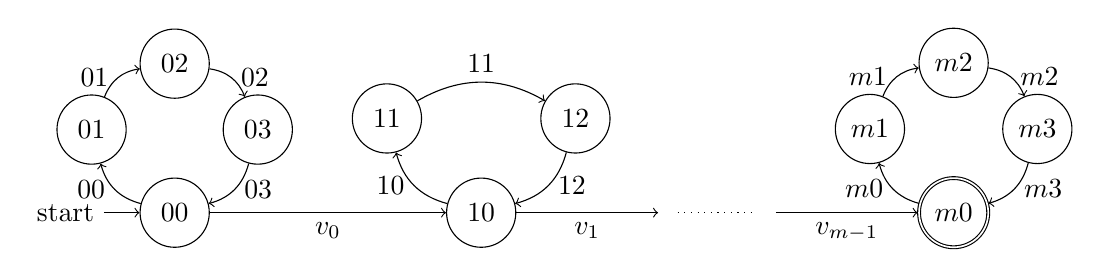
\begin{tikzpicture} 
		\node[state,initial] (q0) {$\st{0}{0}$};
		\node[state] (q1) [right = 3cm of q0] {$\st{1}{0}$};
		\node (q2) [right = 1.8cm of q1]{};
		\node (q3) [right = 1cm of q2]{};
		\node[state,accepting] (qm) [right = 1.8cm of q3] {$\st{m}{0}$};
		
		\node[state] (q01) [above left = 0.6cm of q0] {$\st{0}{1}$};
		\node[state] (q02) [above = 1cm of q0] {$\st{0}{2}$};
		\node[state] (q03) [above right = 0.6cm of q0] {$\st{0}{3}$};

		\node[state] (q11) [above left = 0.8cm of q1] {$\st{1}{1}$};
		\node[state] (q12) [above right = 0.8cm of q1] {$\st{1}{2}$};

		\node[state] (qm1) [above left = 0.6cm of qm] {$\st{m}{1}$};
		\node[state] (qm2) [above = 1cm of qm] {$\st{m}{2}$};
		\node[state] (qm3) [above right = 0.6cm of qm] {$\st{m}{3}$};

 		\draw[->] (q0) edge [bend left] node [left]{$\sym{0}{0}$} (q01) ;
 		\draw[->] (q01) edge [bend left] node [left]{$\sym{0}{1}$} (q02) ;
 		\draw[->] (q02) edge [bend left] node [right]{$\sym{0}{2}$} (q03) ;
 		\draw[->] (q03) edge [bend left] node [right]{$\sym{0}{3}$} (q0) ;
 		
 		\draw[->] (q0) edge node [below]{$v_0$} (q1) ;
 		\draw[->] (q1) edge node [below]{$v_1$} (q2) ;
 		\draw[dotted] (q2) edge (q3) ;
 		\draw[->] (q3) edge node [below]{$v_{m-1}$} (qm) ;

 		\draw[->] (qm) edge [bend left] node [left]{$\sym{m}{0}$} (qm1) ;
		\draw[->] (qm1) edge [bend left] node [left]{$\sym{m}{1}$} (qm2) ;
		\draw[->] (qm2) edge [bend left] node [right]{$\sym{m}{2}$} (qm3) ;
		\draw[->] (qm3) edge [bend left] node [right]{$\sym{m}{3}$} (qm) ;

 		\draw[->] (q1) edge [bend left] node [left]{$\sym{1}{0}$} (q11) ;
		\draw[->] (q11) edge [bend left] node [above]{$\sym{1}{1}$} (q12) ;
		\draw[->] (q12) edge [bend left] node [right]{$\sym{1}{2}$} (q1) ;
	\end{tikzpicture} }
		\caption{An example of a parametric flat automaton}
		\Description{An example of a parametric flat automaton}
			\label{fig:sfa_def}
\end{figure}



The second step of our decision procedure is only enabled if the over-approximation step returns SAT. In this case, our decision procedure uses an under-approximation technique (which is  our main contribution) to restrict the search domain of each string variable to strings that obey some predefined and parameterized pattern.  We propose to use patterns defined by \emph{parametric flat automata} (PFA). A PFA is a {\em flat} finite state automaton consisting of a predefined sequence of loops, each of fixed length (see Figure \ref{fig:sfa_def}). The size of the PFA is parameterized by the length of the sequence of loops and the size of each loop. Adjusting these parameters enlarges or prunes the potential solution space. This approach based on PFA is very flexible yet allows very efficient manipulation. In fact, our procedure restricts the search space for each variable to the set of words accepted by the corresponding given PFA. 


Then, we show that given such restriction, one can  reduce the string constraint solving problem to a linear formula satisfiability problem in polynomial-time. To gain in efficiency, we label each transition  of a PFA with a unique \emph{character} variable (whose domain is the set of natural numbers) instead of having a transition between every two states for each symbol in the alphabet.  This is done by associating to each character in our alphabet a unique natural number. This allows us to avoid the \textit{alphabet explosion problem} from which the approach in~\cite{abdulla2017flatten} suffers and it is  the key for handling string-number conversion efficiently. 




In the following, we explain the construction of the linear formula using $\Phi$ as an example. Assume that we project the domains of $x$ and $y$ to the PFA in Figure~\ref{fig:sfa} (a) and (b), respectively. The variables $v_1$, $v_2$, $v_3$, $v_4$ in the figure are \emph{character} variables. Thus, $v_1$, $v_2$, $v_3$, $v_4$ are also integer variables. For example, from  $ y \in (12)^+$, we may derive $v_2=1$ and $v_3=2$. 

The linear formula produced after the domain restriction will be over variables $v_1$, $v_2$, $v_3$, $v_4$, as well as the number of occurrences of each character variable $\#v_1$, $\#v_2$, $\#v_3$, $\#v_4$. Each model of the linear formula encodes a model of the string constraint. For example, $x=``12"$ and $y=``1212"$ is encoded by the assignment $(v_1,v_2,v_3,v_4,\#v_1,\#v_2,\#v_3,\#v_4) \rightarrow (1,2,1,2,1,1,2,2)$.% 
\footnote{In these examples, we use the shorthand $(x_1,\ldots,x_k)\rightarrow(n_1,\ldots,n_k)$ to denote the function $\{x_1 \mapsto n_1,\ldots, x_k\mapsto n_k\}$.}
The assignment says, for example, that $x$ is the \emph{parametric word} obtained by traversing the loop of $A_x$ once (because $\#v_1 = \#v_2 = 1$), which is $v_1v_2$. Under the assignment $v_1=1$ and $v_2=2$, we obtain $x=``12"$.

If a model of the produced linear formula is found, then the procedure concludes SAT with an assignment to the string variables. If not, our procedure changes the PFAs to a more expressive one (by adding more states and transitions) and repeat the analysis.  We report unknown after failing to prove SAT using a certain number of PFAs.




\begin{figure}
	\tikzset{state/.style={circle,draw=blue!50,fill=blue!20,
			thick,inner sep=0pt,minimum size=6mm}, initial text=$ $}
	
	\begin{minipage}[t]{0.1\textwidth} 
		\scalebox{0.7}{
			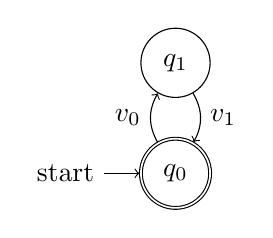
\begin{tikzpicture}
			\node[state,initial,accepting] (q0) {$q_0$};
			
			\node[state] (q01) [above = 0.5cm of q0] {$q_1$};
			
			\draw[->] (q0) edge [bend left] node [left]{$v_0$} (q01) ;
			\draw[->] (q01) edge [bend left] node [right]{$v_1$} (q0) ;
			\end{tikzpicture} }
		
		\centering
		(a) $A_x$
	\end{minipage}
	\begin{minipage}[t]{0.1\textwidth} 
		\scalebox{0.7}{
			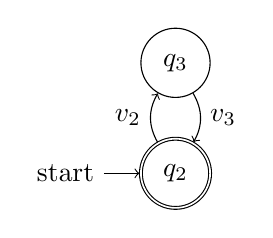
\begin{tikzpicture} 
			\node[state,initial,accepting] (q0) {$q_2$};
			
			\node[state] (q01) [above = 0.5cm of q0] {$q_3$};
			
			\draw[->] (q0) edge [bend left] node [left]{$v_2$} (q01) ;
			\draw[->] (q01) edge [bend left] node [right]{$v_3$} (q0) ;
			\end{tikzpicture} }
		
		\centering
		(b) $A_y$
	\end{minipage}
	\begin{minipage}[t]{0.2\textwidth}
		\scalebox{0.7}{
			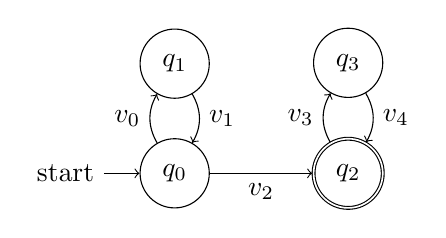
\begin{tikzpicture} 
			\node[state,initial] (q0) {$q_0$};
			\node[state,accepting] (q1) [right = 1.3cm of q0] {$q_2$};
			
			\node[state] (q01) [above = 0.5cm of q0] {$q_1$};
			
			\draw[->] (q0) edge [bend left] node [left]{$v_0$} (q01) ;
			\draw[->] (q01) edge [bend left] node [right]{$v_1$} (q0) ;
			
			\node[state] (q11) [above = 0.5cm of q1] {$q_3$};
			
			\draw[->] (q1) edge [bend left] node [left]{$v_3$} (q11) ;
			\draw[->] (q11) edge [bend left] node [right]{$v_4$} (q1) ;
			\draw[->] (q0) edge node [below]{$v_2$} (q1) ;
			\end{tikzpicture}}
		
		\centering
		(c) $A'_{x}$
	\end{minipage}
			\Description{Examples of parametric flat automata associated to the variables  $x$ and $y$}
	\caption{Parametric flat automata of $x$ and $y$}
	\label{fig:sfa}
\end{figure}






To demonstrate the usefulness of our approach, we have implemented our decision procedure in an open source solver, called {\tool} and evaluated it on a large set of benchmarks obtained from the literature and from symbolic execution of real world programs. The experimental results show that {\tool} is among the best tools for solving basic string constraints and significantly outperforms all other tools on benchmarks with string-number conversion constraints. In this benchmark, the total amount of tests cannot be solved by {\tool} is only a half to the second best tool.



\subsection*{Summary of the Contributions.}

\begin{itemize}

\item An {\em efficient} procedure for checking satisfiability
of string constraints with string-number conversion.



\item The class of \emph{parametric flat automata} which is the key for efficient handling of string constraints.

\item An algorithm that translates the satisfiability problem of string constraints to the satisfiability problem of a linear formula  in polynomial-time when  the search space restricted by PFAs.


\item An open source tool {\tool} with experimental
results that demonstrate the efficiency of
our approach on both existing and real-life benchmarks
\end{itemize}


\subsubsection*{Outline.}
After recalling the  definition in Section \ref{section:sc}, Section \ref{section:over} presents a brief overview of our decision procedure. 
Section \ref{section:sfa} introduces  the class of parametric flat automata. 
Section \ref{section:under_approximate} describes how to use PFA to restrict the searching domain of string variables.
Section \ref{sec:flattening} shows how to construct the linear formula for  basic string constraints (i.e., 
regular, equality, and integer constraints). 
 Section \ref{section:s2i} presents the construction of the linear formula for string-number conversion operations. Section \ref{section:evaluation} presents the details of our implementation and our experimental results.
 Related works are discussed in Section \ref{section:related}. Finally, Section~\ref{section:conclusion} concludes the paper with a discussion of future works.




%%%%%%%%%%%%%%%%%%%%%%%%%%%%%%%%%%%%%%%%%%%%%%%%%%%%%%%%%%%%%%%%%%%%%%%%%%%%%%
\section{Preliminaries} \label{section:preliminary}
%%%%%%%%%%%%%%%%%%%%%%%%%%%%%%%%%%%%%%%%%%%%%

We use $\mathbb{N}$ and $\mathbb{Z}$ to denote the sets of natural numbers and 
integers. For a set $A$, we use $|A|$ to denote its size. 
For $n,m\in\nat$, we write $[n,m]$ for the set of natural numbers 
%(or symbols in $\Sigma$) 
$\{k\mid n\leq k \leq m\}$. 
The function $f$ with the domain restricted to a set $D$ is denoted by $\restrict f D$,
and a set of functions $F$ restricted to a set $D$ is $\restrict F D = \{\restrict f D \mid f \in F\}$.
An \emph{alphabet} is a finite set $\Sigma$ of \emph{characters} and a \emph{word} over $\Sigma$ is a sequence $w = a_1\ldots a_n$ of characters from $\Sigma$, with $\epsilon$ denoting the \emph{empty word}. 
We use $w_1\cdot w_2$ to denote the \emph{concatenation} of words $w_1$ and $w_2$.
$\Sigma^*$ is the set of all words over $\Sigma$, $\Sigma^+ = \Sigma^*\setminus \{\epsilon\}$ and $\Sigma_\epsilon = \Sigma\cup\{\epsilon\}$.
A \emph{language} over $\Sigma$ is a subset $L$ of $\Sigma^*$. 
%
We use $|w|$ to denote the length of $w$ and $|w|_a$ to denote the number of occurrences of the character $a\in \Sigma$ in $w$. 

A \emph{finite automaton} (FA) is a tuple $(Q,T,\Sigma,q_i,q_f)$, where $Q$ is the set of \emph{states}, $T\subseteq Q\times (\Sigma \cup \{\epsilon\}) \times Q $ is the set of \emph{transitions}, $\Sigma$ is the alphabet, $q_i$ is the \emph{initial state}, and $q_f$ is the \emph{final state}. 
A \emph{run} $\pi$ of $A$ over a word $w = a_1\cdots a_n$ is a sequence of transitions $(q_0,a_1,q_1),(q_1,a_1,q_2),\ldots,(q_{n-1},a_n,q_n)$.
 The run $\pi$ (resp. the word $w$) is \emph{accepting} (resp. \emph{accepted}) if $q_0 = q_i$ and $q_n = q_f$.
The \emph{language} of $A$ (denoted by $L(A)$) consists of  the set  of all accepted words.


Through the paper, we will use quantifier-free linear integer arithmetic formulae, and call them \emph{linear formulae} for short.  
Given a linear formula $\phi$ over variables $V$ and an \emph{integer interpretation} of $V$, a function $I:V\rightarrow \integers$, 
we denote by $I\models \phi$ that $I$ satisfies $\phi$ (which is defined in the standard manner), and call $I$ a \emph{model} of $\phi$. 
We use $\modelsof \phi$ to denote the set all models of $\phi$.%



The \emph{Parikh image} of a word $w\in \Sigma^*$ maps each \emph{Parikh variable} $\#a$, with $a \in \Sigma$ is a character, to the number of occurrences of $a$ in $w$.
Formally, given a set $S$, let $\pvarsof S$ denote the set of Parikh variables $\{\#s \mid s\in S\}$. 
The Parikh image of $w$ is a function $\parikhof w:\pvarsof \Sigma \rightarrow \nat$ such that $\parikhof w (\#a) = |w|_a$. 
The Parikh image of a language $L$ is defined as follows $\parikhof L = \{\parikhof w \mid w \in L\}$. %and the Parikh image of an FA $A$ is Parikh image of its language, $\parikhof{A} = \parikhof{L(A)}$. 
%
It is well known that the Parikh image of a regular language  can be  characterized by a linear formula:



\begin{lemma}[\cite{SeidlSMH04}]
Let $A$ be a FA over the alphabet $\Sigma$. Then, we can compute, in linear time,  a linear formula $\parikhfof{A}$, over $\pvarsof \Sigma$, such that $\modelsof{\parikhfof A}_{\#\Sigma} = \parikhof{L(A)}$.
\end{lemma}



 


%%%%%%%%%%%%%%%%%%%%%%%%%%%%%%%%%%%%%%%%%%%%%%%%%%%%%%%%%%%%%%%%%%%%%%%%%%%%%%
\section{String Constraints} \label{section:sc}
%%%%%%%%%%%%%%%%%%%%%%%%%%%%%%%%%%%%%%%%%%%%%%%%%%%%%%%%%%%%%%%%%%%%%%%%%%%%%%


In this section, we formally define string constraints. To begin with, we fix a finite alphabet $\Sigma \subseteq \mathbb{N}$. Note that here we assume that the alphabet is a finite subset of natural numbers. Essentially, we try to capture the numerical encoding of the corresponding symbols in computers (e.g., in ASCII, `A' is encoded as $65$). Hence, we can  assume w.l.o.g. that  there is a one-to-one mapping between numbers in $\Sigma$ and the character it encodes. For the simplicity of presentation, we assume that the character `$0$' is mapped to the number $0$, `$1$' to $1$,$\ldots$, and `$9$' to $9$. For other character $c$, we use $\enc{c}$ to denote the number that it maps to. Notice that this approach is general enough to support any finite set of characters. 


A minor technical difficulty is that sometimes  we may need to treat  $\epsilon$ as a  number. Therefore, we encode $\epsilon$ as some fixed number $\noepsilon\in\nat\setminus\Sigma$.

Assume that $\vars$ ia a set of \emph{string variables} ranging over $\Sigma^*$ and $\varn$ a set of \emph{integer variables} ranging over $\mathbb{Z}$.
An \emph{interpretation over $\vars$ and $\varn$} is a mapping $I:\vars\cup \varn\rightarrow\Sigma^* \cup \mathbb{Z}$. A \emph{word term} is an element in $\vars^*$. We lift the interpretation $I$ to word terms and linear constraints in the standard manner. 

We  use four types of \emph{atomic string constraint}: 
\begin{itemize}

\item An \emph{equality constraint} $\phi_e$ is of the form $t_1 = t_2$ where $t_1, 
t_2$ are word terms. The \emph{model} of $\phi_e$ is the set of interpretations $\modelsof{\phi_e}=\{I\mid 
I(t_1)=I(t_2)\}$. A \emph{disequality constraint} $\phi_d$ is of the form $t_1 \neq 
t_2$ and is interpreted analogously.

\item An \emph{integer constraint} $\phi_i$ is a linear constraint over the integer variables in $\varn$ and values of $|x|$ for all $x \in \vars$, where $|\cdot|:\vars \rightarrow \nat$ is the string length function defined in the standard way.
We define $\modelsof{\phi_i}= \{I \mid I(\phi_i)= \true \}$. 


\item A \emph{regular constraint} $\phi_r$ is of the form $x \in L(A)$ where $x$ is a string variable and $A$ is a finite automaton. The \emph{model} of $\phi_m$ is the set of interpretations $\modelsof{\phi_m}=\{I\mid 
I(x) \in L(A) \}$. 


\item A \emph{string-number conversion constraint} $\phi_s$ is of the form $n=\sti{x}$, where the function $\sti{x}$ is defined as follows. For $a\in [0,9]$, we have $\sti{a}=a$ and for $w \cdot a \in [0,9]^+$, $\sti{w\cdot a} = 10\times \sti{w}+a$. For $w\notin [0,9]^+$, $\sti{w}=-1$. We define $\modelsof{\phi_s}= \{I \mid I(n)= \sti{I(x)} \}$. The \emph{number-string} conversion constraint $x=\its{n}$ is treated as a syntactic sugar for $n=\sti{x}$.

\end{itemize}

A \emph{string constraint} is then a conjunction of atomic string constraints, with the semantics defined in the standard manner. It is \emph{satisfiable} if there is an interpretation which evaluates the  constraint to $\true$. Often we refer to the first three types of atomic string constraints the \emph{basic string constraints}.

Notice that only positive integer is supported in the string-number conversion function. This is the semantics used by most of the SMT solvers, and hence we follow it in this paper. The encoding has a benefit that it can also handle the case where $x$ is ``not a number", using the condition $\sti{x} = -1$.
Supporting only positive integer is not a strong restriction, since converting from negative integer can still be encoded using only the positive  version. 


%%%%%%%%%%%%%%%%%%%%%%%%%%%%%%%%%%%%%%%%%%%%%%%%%%%%%%%%%%%%%%%%%%%%%%%%%%%%%%
\section{Decision Procedure Overview} \label{section:over}
%%%%%%%%%%%%%%%%%%%%%%%%%%%%%%%%%%%%%%%%%%%%%%%%%%%%%%%%%%%%%%%%%%%%%%%%%%%%%%


Our decision procedure has two steps: the first step consists in over-approximating the set of input constraints into a set that falls in the chain-free fragment~\cite{abdulla2019chain}, which is decidable. 
The over-approximation module proceeds as follows: First,  it replaces all string-number conversion constraint $n=\sti{x}$ by $n=-1 \vee (n\neq -1 \wedge x\in [0-9]^*$) to obtain an over-approximation $\Phi$ consisting of only basic string constraints. 
Then, it over-approximates $\Phi$ to a \emph{chain-free string constraint}~\cite{abdulla2019chain}, 
which  consists of only integer, membership, and \emph{chain-free} equality constraints. Informally, a set of equality constraints has a \emph{chain} if we can find some circular dependency between the string variables in the equality constraints.
Our procedure iteratively searches for such dependency chains in the equality constraints. If a chain is found then we replace a variable appearing in that chain by a  fresh one. By doing this, we  break  that chain. We   repeat this procedure until there are no more chains. Observe that if the over-approximation is UNSAT then our decision procedure  declares that the original formula is also UNSAT.




The second step of our decision procedure is only enabled if the over-approximation step returns SAT. In this case, our decision procedure  under-approximates the string constraints by restricting the search domain of each string variable to the language defined by some PFA. This approach based on PFA allows very efficient manipulation. We will show that given such restriction, one can reduce the string constraint solving problem to a linear formula satisfiability problem. The rest of the paper will be mainly dedicated to the explanation of the under-approximation technique (which is our main contribution).




\section{Parametric Flat Automata} \label{section:sfa}
%%%%%%%%%%%%%%%%%%%%%%%%%%%%%%%%%%%%%%%%%%%%%%%%%%%%%%%%%%%%%%%%%%%%%%%%%%%%%%

We introduce \emph{parametric flat automata} that will be used to define patterns used by the under-approximation module to restrict the domain of string variables. 
\scalebox{0.65}{
	\tikzset{state/.style={circle,draw=green!80,fill=green!20,
			thick,inner sep=0pt,minimum size=6mm}, initial text=$ $}

	\renewcommand{\sym}[2]{a_{#1}^{#2}}
	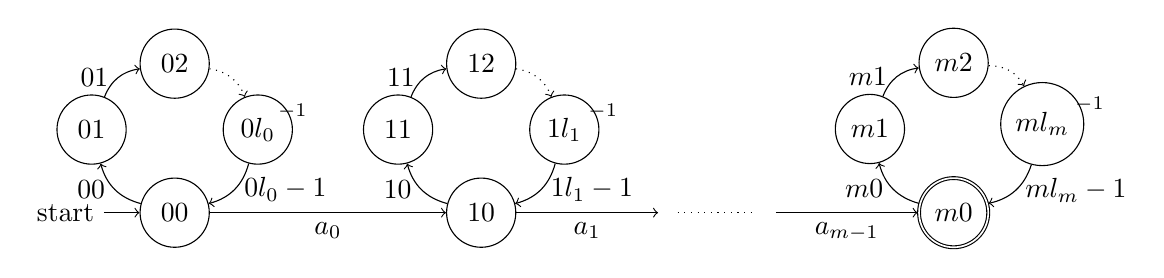
\begin{tikzpicture} 
	\node[state,initial] (q0) {$\st{0}{0}$};
	\node[state] (q1) [right = 3cm of q0] {$\st{1}{0}$};
	\node (q2) [right = 1.8cm of q1]{};
	\node (q3) [right = 1cm of q2]{};
	\node[state,accepting] (qm) [right = 1.8cm of q3] {$\st{m}{0}$};
	
	\node[state] (q01) [above left = 0.6cm of q0] {$\st{0}{1}$};
	\node[state] (q02) [above = 1cm of q0] {$\st{0}{2}$};
	\node[state] (q03) [above right = 0.6cm of q0] {$\st{0}{l_0}$};
	\node   (m1) [above right = -0.4cm and -0.3cm of q03] {$\ ^{-1}$};
	
	\node[state] (q11) [above left = 0.6cm of q1] {$\st{1}{1}$};
	\node[state] (q12) [above = 1cm of q1] {$\st{1}{2}$};
	\node[state] (q13) [above right = 0.6cm of q1] {$\st{1}{l_1}$};
	\node   (m2) [above right = -0.4cm and -0.25cm of q13] {$\ ^{-1}$};
	
	\node[state] (qm1) [above left = 0.6cm of qm] {$\st{m}{1}$};
	\node[state] (qm2) [above = 1cm of qm] {$\st{m}{2}$};
	\node[state] (qm3) [above right = 0.6cm of qm] {$\st{m}{l_m}$};
	\node   (mm) [above right = -0.45cm and -0.2cm of qm3] {$\ ^{-1}$};
	
	\draw[->] (q0) edge [bend left] node [left]{$\sym{0}{0}$} (q01) ;
	\draw[->] (q01) edge [bend left] node [left]{$\sym{0}{1}$} (q02) ;
	\draw[->,dotted] (q02) edge [bend left] node [right]{} (q03) ;
	\draw[->] (q03) edge [bend left] node [right]{$\sym{0}{l_0-1}$} (q0) ;
	
	\draw[->] (q0) edge node [below]{$a_0$} (q1) ;
	\draw[->] (q1) edge node [below]{$a_1$} (q2) ;
	\draw[dotted] (q2) edge (q3) ;
	\draw[->] (q3) edge node [below]{$a_{m-1}$} (qm) ;
	
	\draw[->] (qm) edge [bend left] node [left]{$\sym{m}{0}$} (qm1) ;
	\draw[->] (qm1) edge [bend left] node [left]{$\sym{m}{1}$} (qm2) ;
	\draw[->,dotted] (qm2) edge [bend left] node [right]{} (qm3) ;
	\draw[->] (qm3) edge [bend left] node [right]{$\sym{m}{l_m-1}$} (qm) ;
	
	\draw[->] (q1) edge [bend left] node [left]{$\sym{1}{0}$} (q11) ;
	\draw[->] (q11) edge [bend left] node [left]{$\sym{1}{1}$} (q12) ;
	\draw[->,dotted] (q12) edge [bend left] node [right]{} (q13) ;
	\draw[->] (q13) edge [bend left] node [right]{$\sym{1}{l_1-1}$} (q1) ;	
	

	\end{tikzpicture} }
	
	
\subsubsection*{Flat automata.} 
A finite state automaton  
$A = (Q,T,\Sigma,\st{0}{0},\st{m}{0})$ is said to be \emph{flat} if it satisfies the following structural constraints (see also the figure above):
\begin{enumerate}
	\item The final state $\st{m}{0}$ is reached from  the initial state $\st{0}{0}$ through a straight path of $m-1$ transitions $(\st{i}{0},a_i,\st{i+1}{0}) \in T$ with $\st{i}{0} \in Q$ and $a_i \in \Sigma$ for $i\in[0,m-1]$. 
	\item  
Each state $\st{i}{0}$ is the origin of a unique simple cycle of the length $l_i\in\mathbb{N}$, consisting of states $\st{i}{j-1} \in Q$ and transitions $(\st{i}{j-1}, a_{i}^{j-1}, \st{i}{j \bmod l_i})$, with $a_{i}^{j-1} \in \Sigma$, for $j\in [1,l_i]$. 
Notice that the case when $l_i = 0$ is also admissible and means that there is no cycle on $q_i$.
	\item Each character in $\Sigma$ appears on at most one transition of the automaton $A$. 
\end{enumerate} 

The crucial feature of flat automata is that their semantics can be faithfully represented by a linear formula and handled efficiently by an SMT solver. Such encoding into linear formula results in efficient algorithms and decision procedures. For instance, we avoid dealing with costly standard automata operations (e.g., checking  the non-emptiness of the intersection of several regular languages is known to be {\sc Pspace}-complete while it is in {\sc NP} for the class of flat automata).
The encoding is possible due to the flat structure, which has the property that 
``every word $w\in L(A)$ is uniquely determined by its Parikh image $\parikhof{w}$". 
More precisely, the Parikh image of a word $w\in L(A)$ can be seen as an encoding of $w$ and can be uniquely decoded:


\begin{lemma}\label{lemma:decoding}
For an flat FA $A$, there is a function $\decode A$ such that for each $w\in L(A)$, $\decode A(\parikhof w) = w$. 
\end{lemma}
%
Observe that the $\parikhof w$ value of any variable appearing within  a cycle of $A$ is equal to the number of repetitions of that cycle in the accepting run. This is an immediate consequence of the fact that 
 every character appears on at most one transition. Thus, the accepting run on $w$ (and so $w$ itself) can be reconstructed from $\parikhof w$.  
 
 More concretely, the function $\decode A$ can be implemented as follows. 
Given $\pim:\#\Sigma\rightarrow\nat$,
and assuming that the lengths of the loops of $A$ are $l_0,\ldots,l_{m}$, 
$\decode A(\pim)$ is constructed as the word $w_0 a_{0} w_1 \cdots a_{m-1} w_{m}$ where for each $i\in [0,m]$,
$w_i = (a_i^0 \cdots a_i^{l_{i}-1})^{\pvarsof {a_i^0}}$ if $l_i >0$ and $w_i = \epsilon$ if $l_i = 0$. 

For example, in the automaton given at the beginning of this section, 
from $\parikhwof x {a_0} = \parikhwof x {a_1} = \cdots = \parikhwof x {a_{m-1}}=1$, $\parikhwof x {a^0_1}=\parikhwof x {a^1_1}=\parikhwof x {a^2_1}=2$ and $\parikhwof x {a^i_j}=0$ otherwise,  we derive that $x=a_0(a^0_1a^1_1a^2_1)^2a_1\cdots a_{m-1}$. 

\subsubsection*{Parametric (flat) automata}
Next, we define \emph{parametric automaton} (PA) as a pair  $\pa = (A,\paf)$ where 
$A$ is an automaton operating over an alphabet $\cvar$ of \emph{character variables}  
and $\paf$ is an \emph{interpretation constraint}, a linear formula over $\cvar$. 
\emph{Parametric flat automaton (PFA)} is then a parametric automaton whose  automaton is flat. See Figure~\ref{fig:sfa_def} and~\ref{fig:sfa} for examples of PFAs (without interpretation constraints, i.e., $\paf = \true$.).

Parametric automata accept words over $\cvar$, called \emph{parametric words}, but we still use them as representations of languages over $\Sigma$. 
%
Namely, words over $\cvar$ are interpreted as words over $\Sigma$ under an
\emph{interpretation of $\cvar$},
%
a mapping $I:\cvar\rightarrow\Sigma_\epsilon$ (recall that $\Sigma_\epsilon\defeq \Sigma \cup \{\epsilon\} \subseteq \nat$). 
For a parametric word $x= v_1v_2\cdots v_k$ over $\cvar$, its interpretation $I(x)$ is then defined as $I(v_1)\cdot I(v_2)\cdot \ldots \cdot I(v_k)$.
We then define the semantics of the PA $P$ as the set of strings   
$\semof {\pa} = \{I(x) \mid x\in L(A),I\in\semof \paf\}$ of all interpretations satisfying $\paf$ of all parametric strings in the language of $A$. 

We say that a mapping $I_e:\cvar\cup\#\cvar \rightarrow \nat$ is a \emph{word encoding} of a word $w$  (or a $\pa$-encoding of $w$) if $w$ is an instantiation of some parametric word $x \in L(\pa)$ whose Parikh image and interpretation of character variables are defined by $I_e$.  
%
Conversely, $w$ is a \emph{$\pa$-decoding} of $I_e$.
%
We use $\encode \pa(w)$ below to denote all $\pa$-encodings of a word $w$,
and $\decode \pa (I_e)$ to denote all $\pa$-decodings of a word encoding $I_e$. Namely,  
	$$\encode \pa(w)=\{I_e |  x \in L(\pa), I(x) =w, I\in\semof \paf, I_e = I \cup \parikhof{x}\}$$
	$$\decode \pa(I_e)=\{ w | x \in L(\pa), I(x) =w, I\in\semof \paf, I_e = I \cup \parikhof{x} \}$$

Since a word encoding $I_e$ only records the numbers of occurrences of character variables (Parikh image), 
the same word encoding may be shared by multiple words, as formalized in the definition of $\decode \pa(I_e)$. 

\begin{example}
Let use consider the PFA ${\pa_x}=(A_x,\true)$ from Figure~\ref{fig:sfa}~(a) and let $Y{=}(v_1,v_2,\#v_1,\#v_2)$. Then we have\\
$\encode {\pa_x}( ``aaa" ) =\{ (Y{\rightarrow}(\semof{a},\semof{\epsilon},3,3), Y{\rightarrow}(\semof{\epsilon},\semof{a},3,3)  \}$ and
$\decode {\pa_x}((Y{\rightarrow}(\semof{a},\semof{\epsilon},3,3))=\{``aaa"\} $.
\end{example}

If $\pa$ is a PFA, then by Lemma~\ref{lemma:decoding}, every word encoding $I_e\in \encode \pa( w )$ can be decoded uniquely to the word $w$, i.e.
$$
\{w\} = \decode \pa (\encode \pa (w))
$$

Similarly, as stated by the following corollary of Lemma~\ref{lemma:decoding}, 
Parikh image of parametric words in $L(A)$ paired with character variable interpretations satisfying $\paf$ encode precisely the words in $\semof{\pa}$.





\begin{corollary}\label{corollary:pfa}
For a PFA $\pa = (A,\paf)$,
\\
\centerline{$\semof {\pa} = \decode \pa (\{(I\cup \pim)\mid \pim\in\parikhof{L(A)} ,I\in\semof\paf\})$.}
\end{corollary}

\section{Flat Domain Restriction}
\label{section:under_approximate}

%
In this section, we describe formally how to restrict the domain of string variables to patterns defined by PFA. 
We start the description of the algorithm that converts a string constraint $\insc$ to a linear formula representing the set of solutions under the domain restriction.  
%

The domain restriction is formally defined by restricting the domain of each string variable by a chosen PFA. 
%
Namely, assuming that $X$ is the set of string variables of $\insc$,
a \emph{flat domain restriction} for $\insc$ is a mapping $\dr$ that assigns to each variable $x\in X$, a PFA $\dr(x)$ over character variables $V_x$. Let $V_\dr = \bigcup_{x\in X} V_x$ be the set of all character variables used in $\dr$.
We require that these PFA operate over pairwise disjoint sets of character variables, that is if $x\neq y$ then $V_x \cap V_y = \emptyset$.
%
The particular choice of a PFA 
for each variable depends on the strategy used in the implementation, and will be discussed in Section~\ref{section:evaluation}.
%
The \emph{flattening} of the input string constraint $\insc$, denoted $\underf \dr {\insc}$, will be built inductively following the structure of $\insc$.
For a conjunction of string constraints, we let $\underf \dr {\phi \land \phi'} \defeq \underf \dr {\phi} \land \underf \dr {\phi'}$. We do such decomposition until reached atomic string constraints. We show how to build a flattening $\underf \dr {\phi}$ for every atomic string constraint $\phi$ in the following sections.


The semantics of a string constraint $\phi$ restricted by $\dr$ is then defined as 
$\semof{\phi}^\dr = \{I\in\semof \phi \mid \forall x\in X:I(x)\in\semof{\dr(x)}\}$.

The correctness of the entire construction of $\underf \dr {\insc}$ is expressed by  Theorem~\ref{theorem:correct}. 
It uses the decoding function $\decode \dr$ parameterized by the domain restriction $\dr$. 
Let $Z$ be the set of integer variables in $\insc$.
The function maps an interpretations $I_e$ over $Z\cup V_\dr\cup\#V_\dr$
to an interpretation over $Z \cup X$, following the domain restriction $\dr$. Informally, it ``decodes" an interpretation of integer variables $Z\cup V_\dr\cup\#V_\dr$ to an interpretation of variables in the string constraint $\insc$. Formally,
we define $\decode  \dr (I_e) \defeq \{I \mid \forall z\in Z: I(z) = I_e(z) \wedge\forall x\in X: \{I(x)\} = \decode {\dr(x)} ((I_e)_{V_{\dr(x)}\cup \#V_{\dr(x)}})\}$.
The condition says that (1) $I$ and $I_e$ are consistent over variables in $Z$ and (2) $(I_e)_{V_{\dr(x)}\cup \#V_{\dr(x)}}$ is a word encoding that $\dr(x)$-encodes $I(x)$.
We also define the $\dr$-encoding function as the counterpart of $\dr$-decoding,  
%
namely, for a interpretation $I$ of the string constraint $\insc$,  
we let $\encode \dr (I) =\{I_e\mid \decode \dr (I_e) = \{I\} \}$.
We lift $\decode \dr$ and $\encode \dr$ to sets of interpretations in the standard manner.
\begin{example}
We consider the domain restriction $\dr$ such that $\dr(x)	 =(A_x,\true)$ from Figure~\ref{fig:sfa}~(a) and $\dr(y) = (A_y,\true)$ from Figure~\ref{fig:sfa}~(b). 
Let the set of integer variables be $Z=\{v_z\}$ and let $V_{\dr(x)} =\{v_0, v_1,v_2,v_3\}$. 
For the interpretation $I_e =(v_z,v_0,v_1,v_2,v_3,\#v_0,\#v_1,\#v_2,\#v_3) \rightarrow (3,\semof{a}, \semof{b}, \semof{c},\semof{\epsilon},3,3,2,2)$, we have $\decode \dr (I_e) = \{(z,x,y) \rightarrow(3, ``ababab",``cc") \}$.\\ 
Conversely, for $I=(z,x,y) \rightarrow(3, ``ababab",``cc")$ and $Y=(v_z,v_0,v_1,v_2,v_3,\#v_0,\#v_1,\#v_2,\#v_3)$, we have $\encode \dr (I) =\left\{ 
\begin{array}{l}
Y \rightarrow (3,\semof{a}, \semof{b}, \semof{c},\semof{\epsilon},3,3,2,2), \\
Y \rightarrow (3,\semof{a}, \semof{b},\semof{\epsilon}, \semof{c},3,3,2,2), \\
Y\rightarrow (3,\semof{a}, \semof{b},\semof{c},\semof{c},3,3,1,1)
\end{array}
 \right\}$
\end{example}

\begin{theorem}\label{theorem:correct}
$\decode \dr (\semof {\underf \dr {\insc}}) = \semof{\insc}^\dr$ 
\end{theorem}

The theorem can be proved by a structural induction over $\insc$.
However, for the induction step to go through, we will need to guarantee a stronger correspondence of string constraints $\phi$ and their flattenings $\underf \dr \phi$ than just the semantic equality $\decode \dr (\semof {\underf \dr \phi}) = \semof{\phi}^\dr$.  
Particularly, we will need to
 ensure that $\underf \dr \phi$ captures exactly all $\dr$-encodings of $\semof \phi^\dr$
(indeed, notice that if it would be allowed to capture only some of the encodings, then for instance $\underf \dr {\phi} \land \underf \dr {\phi'}$ could only underapproximate $\semof{\phi\land\phi'}^\dr$).
The inductive argument needed in the correctness proof of the under-approximation then reads as
$$\semof{\underf \dr \phi}_{V_\dr\cup V_{\#\dr}}  = \encode \dr{\semof{\phi}}$$ 
%
In the next sections, 
we will formulate the corresponding correctness lemma for flattening constructed from each type of atomic string constraints.
%
We note that the restriction of $\semof{\underf \dr \phi}$ to $V_\dr\cup V_{\#\dr}$ here is needed since $\underf \dr \phi$ will be constructed with some auxiliary variables. 



\section{Flattening of Basic String Constraints}
\label{sec:flattening}
We will first discuss flattening of the basic string constraints, that is,
regular, equality, and integer constraints. We start by two needed operations over PA, synchronization and concatenation.

\subsubsection*{Synchronization of PAs}
We will now discuss a construction of the \emph{synchronization formula} for two PAs $\pa$ and $\pa'$. 
It is a linear formula $\syncfof \pa {\pa'}$ 
that specifies how each word in the semantic intersection $\semof \pa \cap \semof {\pa'}$ is encoded by $\pa$ and by $\pa'$.
%
More precisely, the models of $\syncfof \pa {\pa'}$ represent pairs of word
encodings 
$I_e$ and $I_e'$ such that $I_e\in\encode \pa(w)$ and $I_e'\in\encode {\pa'} (w)$ (hence $w\in\semof{\pa}\cap\semof{\pa'}$).


Particularly, the synchronization formula is built for two PAs  
$\pa {=} ((Q,T,\cvarone,q_i,q_f),\paf)$ and ${\pa'} {=} ((Q',T',\cvartwo,q_i',q_f'),\paf')$ such that $\cvarone \cap \cvartwo = \emptyset$. 
%
It is extracted from the \emph{asynchronous product} of $\pa$ and $\pa'$. 
%
The asynchronous product is an automaton that uses $Q\times Q'$ as the set of states and 
$\cvarone_\epsilon\times\cvartwo_\epsilon$
as the alphabet. 
%
Every accepting run of $\syncof \pa {\pa'}$ corresponds to a pair of accepting runs, 
a run of $\pa$ over a parametric word $x$ and a run of ${\pa'}$ over a parametric word $x'$. 
The word accepted by the run of $\syncof \pa {\pa'}$ induces constraints on the interpretations of $I$ over $\cvarone$ and $I'$ over $\cvartwo$ under which the two parametric words have the same interpretation, i.e. $I(x) = I'(x')$. 

Intuitively, when the product automaton $\syncof \pa {\pa'}$ takes a transition $((q_1,q_1'), (v,v'),(q_2,q_2'))$, 
it means the character variable $v$ and $v'$ should be assigned the same value,
$\pa$ moves under $v$ from state $q_1$ to state $q_2$ and ${\pa'}$ from $q_1'$ to $q_2'$ under $v'$.
%
When $\syncof \pa {\pa'}$ takes a transition $((q_1,q_1'), (v,\epsilon),(q_2,q_1'))$, 
it means that the character variable $v$ should be assigned $\epsilon$, 
$\pa$ moves under $v$ to $q_1$, and ${\pa'}$ takes no action, since no action is needed to match $\pa$'s reading of $\epsilon$ (hence consumes no symbol from the input word). Symmetrically, ${\pa'}$ might read a variable $v$ assigned $\epsilon$ and $\pa$ may stay.

Formally, the asynchronous product automaton is a tuple $\syncof \pa {\pa'} = (Q\times Q', \syncT, \cvarone_\epsilon \times \cvartwo_\epsilon, (q_i,q_i'),(q_f,q_f'))$, where the transition relation $\syncT$ is the minimal set satisfying the following:
%
\begin{itemize}
\item If $(q_1,v,q_2) \in T$ and $(q_1',v',q_2') \in T'$, then we have $((q_1,q_1'),(v,v'),(q_2,q_2'))\in \syncT$.


\item If $(q_1,v,q_2) \in T$, then for all states $q'\in Q'$, we have $((q_1,q'),(v,\epsilon),(q_2,q'))\in \syncT$.



\item If $(q_1',v',q_2') \in T'$, then for all states $q\in Q$, we have $((q,q_1'),(\epsilon,v'),(q,q_2'))\in \syncT$.
\end{itemize}	
%
The synchronization formula $\syncfof{\pa} {\pa'}$ is extracted from $\syncof \pa {\pa'}$ as follows.
Its first part is the Parikh formula $\parikhfof {\syncof \pa {\pa'}}$ of the product, which encodes all accepting runs of $\syncof \pa {\pa'}$.
%
The second part is a constraint that extracts from a run of $\syncof \pa {\pa'}$ the corresponding runs of $\pa$ and of $\pa'$:
$$ \Psi_{\#} \defeq 
\left(\bigwedge_{v\in\cvarone}\#v = \sum_{x' \in \cvartwo_\epsilon} \#{(v,x')}\right)
\land
\left(\bigwedge_{v'\in\cvartwo} \#v' = \sum_{x \in \cvarone_\epsilon} \#{(x,v')}\right)
$$
Notice that $x,x'$ are either variables or $\epsilon$.
Finally, the third part forces the interpretations of the parametric words accepted by $\pa$ and $\pa'$ to be the same:
$$ \Psi_= \defeq
\bigwedge_{x\in\cvarone_\epsilon,x'\in\cvartwo_\epsilon} \#(x,x')>0 \rightarrow (x=x')
$$
The synchronization formula is then the conjunction 
$$
\syncfof \pa {\pa'} \defeq \parikhfof{\syncof \pa {\pa'}} \land \Psi_{\#} \land \Psi_= \land \paf \land \paf'
$$

The correctness of this construction is stated in Lemma~\ref{lemma:synccorrect} below. 
The correctness of the construction of under-approximations of equality constraints and regular constraints in Section~\ref{section:mem} and Section~\ref{section:eq} rely on it. 
%

\begin{lemma}\label{lemma:synccorrect}
$
\semof {\syncfof \pa {\pa'}}_{\cvarone\cup \cvartwo \cup \pvarone\cup\pvartwo} =
\{I_e\cup I_e'\mid I_e \in \encode \pa (w), I_e'\in\encode {\pa'} (w), w\in\semof \pa \cap \semof {\pa'}\} 
$
\end{lemma}

Informally, the lemma states that the models of $\syncfof \pa {\pa'}$ encode precisely the pairs of equivalent encodings of words from $\semof{\pa}$ and $\semof{\pa'}$, that constitute the intersection $\semof{\pa} \cap \semof{\pa'}$. 
Since that the models of $\syncfof \pa {\pa'}$ include also an assignment to the auxiliary variables of $(\cvarone_\epsilon\times\cvartwo_\epsilon) \cup \pvarsof{(\cvarone_\epsilon\times\cvartwo_\epsilon)}$, the lemma restricts $\semof {\syncfof \pa {\pa'}}$ to ${\cvarone\cup \cvartwo \cup \pvarone\cup\pvartwo}$. 

Notice that if $\pa$ is flat (or, symmetrically, if $\pa'$ is flat), then the semantic intersection $\semof \pa \cap \semof {\pa'}$ can be still decoded from the synchronization formula $\syncfof \pa {\pa'}$. 
Namely, due to Corollary~\ref{corollary:pfa}, we have that if $\pa$ is a PFA, then
$$
\decode \pa (\semof{\syncfof \pa {\pa'}}_{\cvarone\cup \pvarone}) = \semof \pa \cap \semof {\pa'}
$$  

\subsubsection*{Concatenation of PFAs}
Concatenation of PFAs will be needed when flattening equality constraints. Its implementation is straightforward, connect the final state of the first PFA with the initial state of the second by an $\epsilon$-transition. Since our automata do not allow transition directly labeled by $\epsilon$, 
the $\epsilon$-transition is labeled by a fresh variable $v_\epsilon$ forced by the constraint $v_\epsilon = \epsilon$ to take the value $\epsilon$.  

Formally, given PFA $\pa = ((Q,T,\cvarone,q_i,q_f),\paf)$ and ${\pa'} = ((Q',T',\cvartwo,q_i',q_f'),\paf')$ with $Q\cap Q'=\emptyset = \cvarone\cap\cvartwo$, 
their concatenation is the PFA $\pa\cdot \pa' = (Q\cup Q',T\cup T'\cup \{(q_f,v_\epsilon,q_i')\},\cvarone\cup\cvartwo\cup\{v_\epsilon\},q_i,q_f',\paf\land\paf'\land v_\epsilon = \epsilon)$ where $v_\epsilon$ is fresh, not from $\cvarone\cup\cvartwo$. 

\begin{lemma}
%$\semof{\pa\cdot \pa'} = \semof{\pa}\cdot\semof{\pa'}$ and 
$\encode{\pa \cdot\pa'}{(\semof{\pa \cdot \pa})}_{\cvarone\cup \cvartwo \cup \pvarone\cup\pvartwo} =
\{I_e \cup I_e'\mid I_e \in \encode \pa (\semof{\pa}) \wedge I_e' \in\encode {\pa'} (\semof{\pa'})\}$, \mbox{for PFAs $\pa$ and $\pa'$.}
\end{lemma}

With synchronization and concatenation of PA, we are ready to describe flattening of the basic string constraints.

\subsection{Flattening of Regular Constraints} \label{section:mem}

Let us first describe the construction of $\underf \dr {\phi_r}$ for a regular constraint $\phi_r \defeq x \in L(A)$. 
In order to synchronize the FA $A$ with the PFA $\dr(x)$, 
we represent $A$ by a PA $\pa' = (A',\Psi_{\mathit{char}})$.
The automaton $A'$ of $\pa'$ operates over fresh character variables $v_a, a\in\Sigma_\epsilon$, 
and is obtained from $A$ by replacing every occurrence of each character $a\in\Sigma_{\epsilon}$ on a transition by the variable $v_a$. 
The interpretation restriction formula $\Psi_{\mathit{char}}$ of $\pa'$ then binds the fresh character variables to the character values they represent, 
namely, $\Psi_{\mathit{char}} = \bigwedge_{a\in\Sigma_\epsilon} v_a = \semof{a}$. Obviously, $L(A) = \semof{\pa'}$. 
We then let 
$$\underf \dr {\phi_r} = \syncfof{\dr(x)} {\pa'}$$ 

The following lemma states the correctness of this construction. 
It follows from Corollary~\ref{corollary:pfa} and Lemma~\ref{lemma:synccorrect}. 
\begin{lemma}\label{lemma:memcorrect}  $\semof {\underf \dr {\phi_r}}_{V_\dr \cup \#V_{\dr}} = \encode {\dr} (\semof{\phi_r})$ . 
\end{lemma}

\subsection{Flattening of Equality Constraints} \label{section:eq}

We now describe the construction of $\underf \dr {\phi_e}$ for an equality constraint $\phi_e\defeq x_0\cdot x_1 \cdots x_n = x_{n+1}\cdot x_{n+2} \cdots x_m$. 
%
To simplify the presentation, we assume that the variables are pairwise different, i.e. that $i\neq j \implies x_i \neq x_j$. We may make this assumption without loss of generality, since multiple occurrences of variables in $\phi_e$ can be eliminated: whenever $x_i = x_j$ for $i \neq j$, we may replace $x_j$ by a fresh variable $x_j'$ and conjoin the modified $\phi_e$ with a new equality $x_j = x_j'$. 
%
We also assume that all disequality constraint $t \neq t'$ are already converted to equivalent equality constraints and integer constraints in the standard way~\cite{abdulla2015norn}.

Having made these assumptions, we may proceed follows. First, we build two PFAs $\leftA$ and $\rightA$ that encode the left and the right-hand side word term of the equality constraint $\phi_e$, respectively, by concatenating the restrictions of the individual variables. That is
\begin{eqnarray*}
\leftA \defeq& \dr(x_1)\cdot\ldots \cdot \dr(x_n)\\
\rightA \defeq& \dr(x_{n+1})\cdot\ldots \cdot \dr(x_m)
\end{eqnarray*}
The under-approximation of $\phi_e$ is then obtained as their synchronization formula
$$
\underf \dr {\phi_e} = \syncfof \leftA \rightA
$$
The correctness of the construction is stated by the lemma:
\begin{lemma}\label{lemma:eqcorrect}
$\semof {\underf \dr {\phi_e}}_{V_\dr  \cup \#V_\dr} = \encode \dr (\semof{\phi_e})$.
\end{lemma}

\subsection{Flattening of Integer Constraints}
{
\newcommand{\lx}{l_x}
\newcommand{\lv}{l_v}
%Integer constraints are encoded precisely by flattening, not under-approximated. 
Given an integer constraint $\phi_l$ that talks about lengths $|x|$ of string variables $x\in X$. 
We use a version of $\phi_l$ where every occurrence of every length function $|x|$ is replaced by an auxiliary length variable $\lx$ and we add a formula to ensure that the value of $\lx$ is equal to that of $|x|$ even when $x$ is encoded using the character variables $V_x$ and Parikh variables $\# V_x$ of $\dr(x)$.
%
%For every length variable $x\in X$, we add an auxiliary variable $\lx$ that records the length of $x$,   
We will need a set auxiliary variables $\{l_v\mid v\in V_x\}$ to express the length by which the character variable $v$ contributes to the length of an $\dr$-encoded string $x$. 
That is, $\lv$ will be $0$ if $v$ is assigned $\noepsilon$,
otherwise it will equal to the number $\#v$ of its occurrences in the word:
$$
\Psi_{\lv} \defeq (v = \noepsilon \land l_v=0) \lor (v \neq \noepsilon \land l_v = \# v)
$$
The length of the encoded word $x$ is then the sum of the lengths contributed by the individual character variables in $V_x$, 
hence we let 
$$
\Psi_{\lx} \defeq \lx = \sum_{v\in V_x} l_v \land  \bigwedge_{v\in V_x} \Psi_{\lv}\ .
$$
Finally, the linear formula created for $\phi_l$ is 
$$
\underf \dr {\phi_{l}} \defeq \phi_l \land \bigwedge_{x\in X} \Psi_{\lx}
$$
and the following lemma states its correctness.
}
\begin{lemma}\label{lemma:eqcorrect}
$\semof {\underf \dr {\phi_l}}_{V_\dr  \cup \#V_\dr} = \encode \dr (\semof{\phi_l})$
\end{lemma}

\hide{The length of $x$ can be specified by the following formula.

$\begin{array}{ccc}
	(|x|&=& \#(v_0)+1 \wedge 0\leq v_1 \leq 9 \wedge v_2 = -1)\vee \\
	(|x|&=& \#(v_0)+2 \wedge 0\leq v_2 \leq 9 \wedge v_3 = -1)\vee \\
	& &\ldots\\
	(|x|&=& \#(v_0)+(m-1) \wedge 0\leq v_{m-1} \leq 9 \wedge v_m = -1)\vee\\
	(|x|&=& \#(v_0)+m \wedge 0\leq v_m \leq 9 )
\end{array}$}




%%%%%%%%%%%%%%%%%%%%%%%%%%%%%%%%%%%%%%%%%%%%%%%%%%%%%%%%%%%%%%%%%%%%%%%%%%%%%%
\section{Flattening of String-Number Conversion} \label{section:s2i}
%%%%%%%%%%%%%%%%%%%%%%%%%%%%%%%%%%%%%%%%%%%%%%%%%%%%%%%%%%%%%%%%%%%%%%%%%%%%%%

Last, we present the main contribution of this paper, 
the construction of a flattening $\underf \dr {\phi_s}$ of string-number conversion constraint $\phi_s \defeq n=\sti{x}$. 

Let us begin with a simple example. Assume that we use the PFA in Figure~\ref{fig:sfa} (a) to restrict the domain of $x$. Then we know that when $0\leq v_0,v_1 \leq 9$, then $n$ is a positive integer value, and otherwise $n =-1$. So we should first add the constraint $ ((0\leq v_0\leq 9) \wedge (0\leq v_1\leq 9)) \vee (n=-1 \wedge (v_0 >9 \vee v_1 >9))$.

For the case that $n$ is a positive integer, the value of $n$ can be characterized by a constraint (assume character variables are not assigned $\epsilon$) $n= (v_0\times 10+ v_1) \times (1+100 +100^2 + \ldots 100 ^{\#v_0-1})=  (v_0\times 10+ v_1) \times \frac{100^{\#v_0}-1}{100-1}$. 
The constraint uses $\#v_0$ to capture the total number of loop traversals.
Notice that the constraint above contains an exponential component $\frac{100^{\#v_0}}{100-1}$. To solve the satisfiability of this formula, one needs to solve an exponential constraint. 

Let us have a look at another example. If we restrict the domain of $x$ to the PFA in Figure~\ref{fig:sfa} (c), for the case when $n$ is positive, we have the relation $n= (v_0 \times 10+ v_1) \times (1+100 +100^2 + \ldots 100 ^{\#v_0-1})\times 10\times 100^{\#v_3}+ v_2 \times 100^{\#v_3}  +(v_3\times 10+ v_4) \times (1+100 +100^2 + \ldots 100 ^{\#v_3-1}) =  (v_0\times 10+ v_1) \times \frac{100^{\#v_0-1}}{100-1}\times 10\times 100^{\#v_3} + v_2 \times 100^{\#v_3}+ (v_3\times 10+ v_4) \times \frac{100^{\#v_3-1}}{100-1}$. Observe that the formula has multiple exponential components, including $\frac{100^{\#v_0}\times 100^{\#v_3} }{100-1}$ and $\frac{100^{\#v_3} }{100-1}$.

It is not difficult to see from the examples above that, if $\dr(x)$ is an arbitrary PFA with $m$ loops, the formula that defines the number $n$ contains at least $m$ exponential components, one for each loop.
To the best of our knowledge, the satisfiability problem of integer constraints with a mix of polynomials and exponentials is still open. The problem is difficult even for the case that variables are real numbers. For example, the algorithm in~\cite{kincaid2019closed} involves a quantifier elimination procedure which is double-exponential to the length of the input formula and hence cannot handle large instances. We therefore do not expect that such constraint can be solved efficiently. Instead, we will define a special form of the flat restriction $\dr(x)$ of $x$ that leads to an easier linear formula.

\subsubsection*{PFA that allows efficient string-number conversion: } 
We will now discuss the special form of $\dr(x)$, called \emph{numeric PFA}, which we choose for string variables appearing in string-integer constraints and that leads to efficient under-approximation technique.
%
Besides simple induced linear formulae, we still want single $\dr(x)$ to cover as many numerals as possible.
We want an ``easy" completeness property, that is,  (1) the space of all numerals can be covered completely by our special numeric PFAs, (2) these numeric PFAs are generated easily, and (3) each of them covers a large and practically significant portion of numerals (so that satisfiable assignments can be often found within the domain restriction of just few of numeric PFAs).
%
Particularly, we will proceed towards a definition of \emph{numeric PFA} $(A^m,\paf^m),m\in\nat$ which covers all numerals that encode integers with $m$ digits.

Our first attempt is a PFA without loop, i.e., a straight line structure 
\scalebox{0.5}{\tikzset{state/.style={circle,draw=blue!50,fill=blue!20,
			thick,inner sep=0pt,minimum size=6mm}, initial text=$ $}
	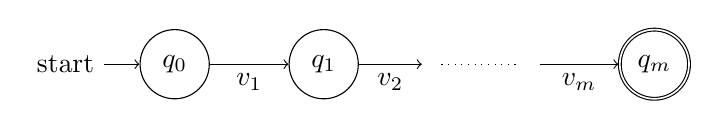
\begin{tikzpicture} 
		\node[state,initial] (q0)  {$q_0$};
		\node[state] (q1) [right = 1cm of q0] {$q_1$};
		\node (q2) [right = 0.8cm of q1]{};
		\node (q3) [right = 1cm of q2]{};
		\node[state,accepting] (qm) [right = 1cm of q3] {$q_m$};
		
		\draw[->] (q0) edge node [below]{$v_1$} (q1) ;
		\draw[->] (q1) edge node [below]{$v_2$} (q2) ;
		\draw[dotted] (q2) edge (q3) ;
		\draw[->] (q3) edge node [below]{$v_m$} (qm) ;
	\end{tikzpicture}}
. The corresponding integer constraint does not have exponential components. However, it does cover all numbers with at most $m$-digits. Consider the example $\sti{x}=10 \wedge |x|=5$. The number $10$ has only $2$-digits, at the first glance, a straight-line PFA with two transitions, i.e., the PFA
    \scalebox{0.5}{\tikzset{state/.style={circle,draw=blue!50,fill=blue!20,
			thick,inner sep=0pt,minimum size=6mm}, initial text=$ $}
	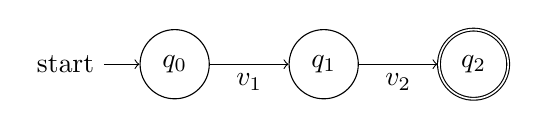
\begin{tikzpicture} 
	\node[state,initial] (q0)  {$q_0$};
	\node[state] (q1) [right = 1cm of q0] {$q_1$};
	\node[state,accepting] (q2) [right = 1cm of q1] {$q_2$};
	
	\draw[->] (q0) edge node [below]{$v_1$} (q1) ;
	\draw[->] (q1) edge node [below]{$v_2$} (q2) ;
	\end{tikzpicture}
	} should be sufficient for the domain restriction of $x$. If we do so, we will conclude that the formula is unsatisfiable, because the length of $x$ cannot be $5$  under this domain restriction.

However, the formula is satisfiable when $x=``00010"$. Observe that $\sti{``00010"}=10$ \changed{since PFAs accept  numeric words with least significant bit first}. The key is that even for a bounded integer, the corresponding numeral can be of an unbounded length with arbitrarily many trailing `$0$'s at the front. All numbers with up to $m$-digits can be however still handled without having to solve exponential constraints. It is enough to equip the initial state of the PFA with a  $0$-self-loop.

Consequently, the automaton $A^m$ of our number PFA will have the following form illustrated in Figure~\ref{fig:sfa_its}. 
It has a self-loop on the initial state labeled by the character variable $v_0$, 
forced by the constraint 
$$
\Psi_{v_0}\defeq v_0=0
$$ 
to hold the value $0$. 
This transition ensures that the under-approximation handles numerals with arbitrary number of trailing zeros.  
The self-loop is followed by a chain of $m$ transitions $(q_{i-1},v_i,q_{i}),1\leq i \leq m$, leading towards the final state $q_m$. 
The chain encodes at most $m$ meaningful digits (only \emph{at most} because the first variables in the sequence can still be assigned zeros and some variables may be assigned $\epsilon$). Hence this PFA covers all numerals that encode numbers with at most $m$ digits.
Although it still has a loop, it will not create any exponential component defining the value of $n$ because the loop only represents a sequence of ``0" at the front of $x$. Thus, it will not affect the integer value of $n=\sti{x}$.

\begin{figure}
	\scalebox{0.7}{
	\tikzset{state/.style={circle,draw=blue!50,fill=blue!20,
			thick,inner sep=0pt,minimum size=6mm}, initial text=$ $}
	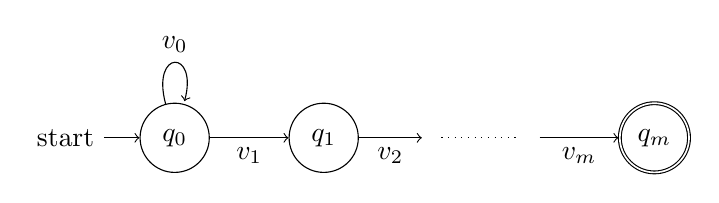
\begin{tikzpicture} 
	\node[state,initial] (q0)  {$q_0$};
	\node[state] (q1) [right = 1cm of q0] {$q_1$};
	\node (q2) [right = 0.8cm of q1]{};
	\node (q3) [right = 1cm of q2]{};
	\node[state,accepting] (qm) [right = 1cm of q3] {$q_m$};
	
	\draw[->] (q0) edge node [below]{$v_1$} (q1) ;
	\draw[->] (q1) edge node [below]{$v_2$} (q2) ;
	\draw[dotted] (q2) edge (q3) ;
	\draw[->] (q3) edge node [below]{$v_m$} (qm) ;
	\path (q0) edge [loop above] node {$v_0$} (q0);
	\end{tikzpicture} }
	
	\caption{PFA for string-number conversion constraints}
	\label{fig:sfa_its}
	\Description{Parametric flat automata  for string-number conversion constraints}
\end{figure}


Numeric PFA with these restrictions would satisfy our primary objective, that is, they would induce linear formulae and would ``easily" and completely cover all numerals.
%
A last problem still needs to be solved before they can be efficient in practice. 
%
Recall that the character variables can be assigned $\epsilon$.  
%
Therefore, a single chain of $k$ interesting digits, $k\leq m$, can be by $A^m$ represented in $k\choose m$ ways, each corresponding to one possible interleaving of $k$ digits with $m-k$ epsilons. 
%
%\lh{I am not sure whether it is really impossible to make a small formula}
%
This may  lead to a formula of   exponential size  when defining  the value of $n$.
%
In order to eliminate this potential blow-up in the size of the formula, we add to $\paf^m$ an additional constraint that forces all epsilons to be \emph{shifted} behind the least significant digit. This will leave us with only one interleaving. This is the formula
$$
\Psi_{\mathsf{shift}}^m \defeq \bigwedge_{1\leq i \leq m} v_i \neq \noepsilon \implies v_{i-1}\neq \noepsilon \ .
$$
Last, since this restriction is meaningful only when the string is indeed a numeral,  
we also define the constraint representing the strings which are not numerals, the formula
$$
\Psi_{\mathsf{NaN}}^m \defeq  \bigvee_{i\in [1,m]} v_i>9
$$ 
and define the final form of the interpretation restriction used by $A^m$ as 
$$
\paf^m \defeq  \Psi_{\mathsf{NaN}}^m \lor (\Psi_{v_0} \land \Psi_{\mathsf{shift}}^m)\ .
$$
Consequently, we design our domain restrictions $\dr$ so that for string variables $x$ that appear within string-integer constraints,  $\dr(x)$ is a number PFA $(A^m,\paf^m),m\in \nat$. 

Assuming that the domain restriction for $x$ is $(A^m,\paf^m)$, 
the value of the integer $n$ can be extracted from a numeral using the formula
$$
\Psi_{\mathsf{toInt}}^m\defeq \bigvee_{1\leq k \leq m} \Psi_{\mathsf{last(k)}}^m \land (n = v_1* 10^{k-1} + v_2* 10^{k-2} + \ldots + v_{k})
$$
where $\Psi_{\mathsf{last(k)}}^m$ says that the last variable of $A^m$ assigned a non-$\epsilon$ value is $v_{k}$, namely 
$$
\Psi_{\mathsf{last(k)}}^m \defeq (k = m \land v_k \geq 0) \lor (v_{k} \geq 0 \land v_{k+1} = -1)\ .
$$
Since we also need to distinguish the case when $x$ is not a number, in which case $n$ should equal $-1$, 
the formula under-approximating $\phi_s$ is finally constructed as  
\begin{multline*}
\underf \dr {\phi_s} 
\defeq 
\parikhfof{A^m} 
\land \\
\bigl((\Psi_{\mathsf{NaN}}^m \land n = -1) 
\lor 
(\neg\Psi_{\mathsf{NaN}}^m \land \Psi_{\mathsf{toInt}}^m)\bigr)
\end{multline*}
The following lemma states correctness of this construction:
\begin{lemma}
$
\semof {\underf \dr {\psi_s} }_{V_\dr \cup \#V_\dr} = \encode  \dr(\semof{\phi_s})
$
\end{lemma}



\section{Implementation and Evaluation}
\label{section:evaluation}

We have implemented our string constraint solving procedure in a tool called {\tool}. {\tool} is implemented as a theory solver of the SMT solver Z3~\cite{z3}. In this way, we can concentrate on solving conjunctive constraints and let Z3 handle the other boolean connectives. Secondly, it makes it possible to solve not only formulae over string constraints but also combinations of string constraints with other theories that Z3 supports. Furthermore, this approach allows us to more effectively handle the arithmetic constraints that are generated by the under-approximation module and, lastly, it eliminates the need to have our own parser. 

In {\tool}, we use the following PFA selection strategy. We use \emph{numeric PFAs} for string variables appearing in string-number conversion and \emph{standard PFAs} for others. We select a size $m$ for numeric PFAs, a number $p$ of their loops, and the length $q$ of the loops. Initially, we set $(m,p,q)=(5,2,q)$ where $q$ is dynamic and obtained from our internal static analysis. We double $m$ and increase $p$ and $q$ by one if refinement is required. We set an upper bound for each parameter and report UNKNOWN if a solution cannot be found within the bound.

Our over-approximation module also uses heuristics to derive the constant value of any side of the constraint $n=\sti{x}$ to refine the over-approximation. For instance, assume we can derive that $n=12$ from some integer constraints. Then we can derive the value of $x$ belongs to the regular language $(0^*12)$. 
%HERE

%more or less standard
The way our theory solver and Z3 interact is almost standard. When Z3 asks our theory solver a string constraint satisfiability problem, our solver tries to prove it is SAT or UNSAT using the procedure discussed in this paper. For under-approximation, whenever a corresponding linear formula is created, we attach the current value of $m$, $p$, $q$ to the formula, and then push it to Z3 core. If our theory solver reports UNKNOWN, Z3 remembers it in a global flag \textsf{incomplete} and either tries another solution branch, or the same solution branch with different value of $m$, $p$, $q$. If Z3 completes the search of all solution branches, it reports UNSAT if the flag \textsf{incomplete} is down, and UNKNOWN otherwise.


We compare {\tool} \changed{(\texttt{1e715b7dab})} with other state-of-the-art string solvers, namely, CVC4~(45bcf28ab)~\cite{cvc4Tool}, and Z3~(\texttt{d95b549ff})~\cite{z3}, \textsf{Z3Str3}~(\texttt{d95b549ff})~\cite{zheng2013z3}. For these tools, we use the GitHub version stated in the parenthesis because their performance are in general better than the corresponding release version. \changed{Observe that CVC4 and Z3 are  DPLL(T)-based string solvers.}
We do not compare with Sloth \cite{sloth} since it does not support length constraints, which occur in most of our benchmarks. We also do not compare with ABC~\cite{aydin2018parameterized} (a model counter for string constraints), Ostrich~\cite{chen2019decision} and \textsf{Trau+}~\cite{abdulla2019chain}, because they do not support many of the string functions in our benchmarks, especially string-number conversion.

We perform two sets of experiments. In the first set of experiments, we compare {\tool} with other tools on existing benchmarks over basic string constraints. Those benchmarks do not involve string-number conversion functions. In the second set of experiments, we compare {\tool} with the other tools on new suites focusing on string-number conversion. Our goals of experiments are the following:
\smallskip


\begin{itemize}
	\item {\tool} performs as good as or better than the other tools in solving the  satisfiability problems of basic string constraints.
	
		\smallskip

	\item {\tool} performs significantly better than the other tools in solving the satisfiability problems on string-number conversion benchmark, and this shows  the efficiency of PFA in general and \emph{numeric} PFA in particular.
\end{itemize}
		\smallskip

In the first set of experiments, we use the following benchmark examples:

		\smallskip


\begin{itemize}
	\item PyEx~\cite{pyex} comes from running the symbolic executor PyEx over some Python packages.
	
	\smallskip
	
	
%	\item APLAS~\cite{aplas} includes 600 hand-drafted tests consisting of only equality and integer length constraints.
	
	
	%	\smallskip


	\item \changed{ LeetCode comes from running PyEx over a sample code collected from the LeetCode~\cite{LeetCode} website, including functions that check whether a string is a valid IPv4 or IPv6 address, sum up two binary numbers, check whether an input string is an abbreviation of another input string, and convert a sequence of digits to a string according to a given mapping.}
	
		\smallskip

	\item StringFuzz~\cite{blotsky2018stringfuzz}  is generated by the fuzz testing tool of the same name.
	
		\smallskip

	\item $\text{cvc4}_{\text{pred}}$ and $\text{cvc4}_{\text{term}}$ are obtained from the CVC4 group~\cite{termEQ}. These benchmarks contain a small amount of string-number conversion constraints (< $5\%$).
\end{itemize}

In the second experiment, we compare with tools supporting string-number conversion on the benchmarks collected from the symbolic executor \texttt{Py-Conbyte}\footnote{\url{https://github.com/spencerwuwu/py-conbyte}}, which has the supports of string-number conversion. We ran it on several examples collected from the LeetCode platform and from Python core libraries, which involve diverse usages of string-number conversion in Python such as parsing date-time, verifying and restoring IP addresses from strings, etc. We also have examples that encode execution paths of some JavaScript programs (the Luhn algorithm and some array manipulations).

	\changed{All experiments were executed on a machine with 4-core CPU, 16 GiB RAM, and MacOS 10.15.4.} The timeout was set to 10s for each test.
We use the results from {\tool}, CVC4, and Z3 as the reference answer for the validation of the correctness of the results. Occasionally, two of them report inconsistent  answers (one SAT and one UNSAT). To decide which solver is right, we developed a validator. It takes the model $I$ returned from the solver who reported SAT, assigns $I(x)$ to all variables $x$ in the test to obtain a modified test, and re-evaluates the modified test by multiple solvers. If the results from all solvers are consistent, we mark the test SAT or UNSAT according to the results. Otherwise, we manually simplify and inspect the test until we get a conclusive result. 

\changed{The results of the experiments are summarized in Table~\ref{table:base_benchmark}, Table~\ref{table:str_int_benchmark}, and Table~\ref{table:checkLuhn}. Rows with heading \texttt{SAT}/\texttt{UNSAT} show numbers of solved formulae. Rows with heading \texttt{UNKNOWN} or \texttt{TIMEOUT} indicate the number of instances for which the solver fails to return an answer. \texttt{ERROR} means system crashes due to various reasons (usually out of memory). \texttt{INCORRECT} shows the number of cases where the tool gives a wrong answer.}


\begin{table}[h]
\changed{
\centering
\caption{Results of {\tool}, CVC4, Z3, and Z3Str3 on Basic String Constraint benchmarks.}
\scalebox{0.85}{
\begin{tabular}{|l r | r r r r |}
\hline
\multicolumn{2}{|c}{}                  & {\tool} & CVC4  &Z3 & Z3Str3 \\ \hline
\multirow{6}{*}{PyEx}		& SAT      & 21377& 19899& 16331&  3037 \\
							& UNSAT    &  3860&  3848&  3831&  3816 \\
							& UNKNOWN  &     0&     0&     0&     7 \\
							& TIMEOUT  &   184&  1674&  5259& 16872 \\
							& ERROR    &     0&     0&     0&  1675 \\
							& INCORRECT&     0&     0&     0&    14 \\ \hline
%\multirow{6}{*}{APLAS}		& SAT      &   126&    51&    13&    35 \\
%							& UNSAT    &   286&   214&   100&   111 \\
%							& UNKNOWN  &     0&     0&     0&   345 \\
%							& TIMEOUT  &   188&   335&   487&    89 \\
%							& ERROR    &     0&     0&     0&    20 \\
%							& INCORRECT&     0&     0&     0&     0 \\ \hline
\multirow{6}{*}{LeetCode}	& SAT      &   877&   865&   881&   661 \\
							& UNSAT    &  1785&  1785&  1785&  1780 \\
							& UNKNOWN  &     0&     0&     0&   122 \\
							& TIMEOUT  &    0&    16&     0&    90 \\
							& ERROR    &     4&     0&     0&    13 \\
							& INCORRECT&     0&     0&     0&     0 \\ \hline
\multirow{6}{*}{StringFuzz}	& SAT      &   515&   704&   267&   505 \\
							& UNSAT    &   301&   245&   188&   192 \\
							& UNKNOWN  &     0&     0&     0&     4 \\
							& TIMEOUT  &   249&   116&   610&   364 \\
							& ERROR    &     0&     0&     0&     0 \\
							& INCORRECT&     0&     0&     0&     0 \\\hline
\multirow{6}{*}{cvc4\textsubscript{pred}} & SAT &    13&    11&    12&     8 \\
							& UNSAT    &   822&   818&   808&   774 \\
							& UNKNOWN  &     0&     0&     0&     4 \\
							& TIMEOUT  &     0&     6&    15&    38 \\
							& ERROR    &     0&     0&     0&     11 \\
							& INCORRECT&     0&     0&     0&     0 \\ \hline
\multirow{6}{*}{cvc4\textsubscript{term}} & SAT &    10&     8&     5&    2 \\
							& UNSAT    &  1032&  1025&  1022&   957 \\
							& UNKNOWN  &     0&     0&     0&     3 \\
							& TIMEOUT  &     3&    12&    18&    58 \\
							& ERROR    &     0&     0&     0&     11 \\
							& INCORRECT&     0&     0&     0&    14 \\ \hline \hline
\multirow{6}{*}{Total} 		& SAT      & 22792& 21487& 17496&  4213\\
							& UNSAT    &  7800&  7721&  7634&  7519\\
							& UNKNOWN  &     0&     0&     0&   140\\
							& TIMEOUT  &  436&  1824&  5902& 17422 \\
							& ERROR    &     4&     0&     0&  1710\\
							& INCORRECT&     0&     0&     0&    28 \\\hline
\end{tabular}}
\label{table:base_benchmark}}
\end{table}

\begin{table}[h]
\changed{
\centering
\caption{Results of {\tool}, CVC4, Z3, and Z3Str3 on String-Number Conversion benchmark.}
\scalebox{0.8}{
\begin{tabular}{|l r | r r r r|}
\hline
\multicolumn{2}{|c}{}          			   & {\tool} &  CVC4 &    Z3 & Z3Str3 \\ \hline
\multirow{6}{*}{Leetcode}		& SAT      &  2501&  1721&  1898&   239 \\ 
								& UNSAT    & 16394& 15726& 16115& 15288 \\
								& UNKNOWN  &     0&     0&     0&   623 \\
								& TIMEOUT  &    32&  1480&   914&  2337 \\
								& ERROR    &     0&     0&     0&   332 \\
								& INCORRECT&     0&     0&     0&   108 \\ \hline 
\multirow{6}{*}{PythonLib}		& SAT      &  1922&   579&   914&   206 \\ 
								& UNSAT    &   724&   667&   724&   642 \\
								& UNKNOWN  &     0&     0&     0&    45 \\
								& TIMEOUT  &     0&  1400&  1008&  1710 \\
								& ERROR    &     0&     0&     0&    41 \\
								& INCORRECT&     0&     0&     0&     2 \\ \hline
\multirow{6}{*}{JavaScript}		& SAT      &    20&     3&    16&     4 \\ 
								& UNSAT    &     0&     0&     0&     0 \\
								& UNKNOWN  &     0&     9&     0&     0 \\
								& TIMEOUT  &     0&     8&     4&    10 \\
								& ERROR    &     0&     0&     0&     6 \\
								& INCORRECT&     0&     0&     0&     0 \\ \hline \hline
\multirow{6}{*}{Total}			& SAT      &  4443&  2303&  2828&   449 \\ 
								& UNSAT    & 17118& 16393& 16839& 15930 \\
								& UNKNOWN  &     0&     9&     0&   668 \\
								& TIMEOUT  &    32&  2888&  1926&  4057 \\
								& ERROR    &     0&     0&     0&   379 \\
								& INCORRECT&     0&     0&     0&   110 \\ \hline
\end{tabular}}
\label{table:str_int_benchmark}
}
\end{table}


% \begin{table}[h]
% \centering
% \caption{Results of {\tool}, CVC4, Z3, and Z3Str3 on Basic String Constraint benchmarks.}
% \scalebox{0.85}{
% \begin{tabular}{|l r | r r r r |}
% \hline
% \multicolumn{2}{|c}{}                  & {\tool} & CVC4  &Z3 & Z3Str3 \\ \hline
% \multirow{3}{*}{PyEx}		& SAT      &  19468  & 19763 & 16528 &  3030 \\ 
% 							& UNSAT    &   3854  &  3834 &  3831 &  3836 \\
% 							& $\times$ &   2099  &  1824 &  5062 & 18555 \\ \hline
% \multirow{3}{*}{APLAS}		& SAT      &    131  &   205 &    12 &    37 \\
% 							& UNSAT    &    288  &   221 &   100 &   111 \\
% 							& $\times$ &    181  &   174 &   488 &   452 \\ \hline
% \multirow{3}{*}{LeetCode}	& SAT      &    881  &   859 &   881 &   670 \\
% 							& UNSAT    &   1785  &  1785 &  1785 &  1780 \\
% 							& $\times$ &      0  &    22 &     0 &   216 \\ \hline
% \multirow{3}{*}{StringFuzz}	& SAT      &    498  &   671 &   264 &   491 \\
% 							& UNSAT    &    319  &   240 &   186 &   192 \\
% 							& $\times$ &    248  &   154 &   615 &   382 \\\hline
% \multirow{3}{*}{cvc4\textsubscript{pred}} & SAT & 11 & 11 &   12 &     8 \\
% 							& UNSAT    &    820  &   818 &   808 &   772 \\
% 							& $\times$ &      4  &     6 &    15 &    55 \\ \hline
% \multirow{3}{*}{cvc4\textsubscript{term}} & SAT & 13 & 8 &     5 &    17 \\
% 							& UNSAT    &   1031  &   936 &  1021 &   958 \\
% 							& $\times$ &      1  &   101 &    19 &    70 \\ \hline \hline
% \multirow{3}{*}{Total} 		& SAT      &  21002  & 21517 & 17702 &  4253 \\
% 							& UNSAT    &   8097  &  7834 &  7731 &  7649 \\
% 							& $\times$ &   2533  &  2281 &  6199 & 19730 \\\hline	
% \end{tabular}}
% \label{table:base_benchmark}
% \end{table}

% \begin{table}[h]
% \centering
% \caption{Results of {\tool}, CVC4, Z3, and Z3Str3 on String-Number Conversion benchmark.}
% \scalebox{0.8}{
% \begin{tabular}{|l r | r r r r|}
% \hline
% \multicolumn{2}{|c}{}          			   & {\tool} & CVC4  &    Z3  & Z3Str3 \\ \hline
% \multirow{3}{*}{Leetcode}		& SAT      &   2349  &  1543 &  1892  &   217 \\ 
% 								& UNSAT    &  16368  & 15676 & 16105  & 15374 \\
% 								& $\times$ &    210  &  1708 &   930  &  3336 \\ \hline 
% \multirow{3}{*}{PythonLib}		& SAT      &    886  &   408 &   797  &   201 \\ 
% 								& UNSAT    &    720  &   660 &   724  &   644 \\
% 								& $\times$ &   1040  &  1578 &  1125  &  1801 \\ \hline
% \multirow{3}{*}{JavaScript}		& SAT      &     20  &     6 &    16  &     4 \\ 
% 								& UNSAT    &      0  &     0 &     0  &     0 \\
% 								& $\times$ &      0  &    14 &     4  &    16 \\ \hline \hline
% \multirow{3}{*}{Total}			& SAT      &   3255  &  1957 &  2705  &   422 \\ 
% 								& UNSAT    &  17088  & 16336 & 16829  & 16018 \\
% 								& $\times$ &   1250  &  3300 &  2059  &  5153 \\ \hline
% \end{tabular}}
% \label{table:str_int_benchmark}
% \end{table}


From Table~\ref{table:base_benchmark}, we can see that the performance of {\tool} is as good as that of the most competitive tools such as CVC4 and Z3 on basic string constraints. In all of the benchmarks, {\tool} ranked either the 1st or the 2nd on the number of solved (SAT+UNSAT) cases. On the StringFuzz benchmarks that are SAT, {\tool} does not perform as well as the best performing tool. We however do not consider this crucial because these benchmarks are just randomly generated for debugging. On the most important benchmarks, those that come from program analysis, {\tool} is comparable to the best performing tool.

%\changed{
%From Table~\ref{table:str_int_benchmark}, we can see that {\tool} significantly outperforms all the other tools. 
%The second best tool, Z3, fails on 38\% more examples. 
%}
\changed{
From Table~\ref{table:str_int_benchmark}, we can see that {\tool} significantly outperforms all the other tools. 
The second best tool, Z3, fails on 50 times more examples. 
}
%It fails on twice less cases then Z3, which is ranked the 2nd. In fact, most of the failed tests come from the analysis of one Python core library function that converts an IPv6 address to a number. From around 2028 tests generated from this function, around 1000 tests are too difficult for all solvers.  If we exclude the 2028 tests generated from this function, then {\tool} has only $218$ failed cases in total. This is significantly better than the 2nd place tool Z3, which fails on $942$ cases in total.

%We also ran experiments on the String-Number Conversion benchmark with the timeout set to 30s. Provided more time for solving, {\tool} managed to obtain more results and the number of failed cases is reduced to 539, while CVC4 and Z3Str3 got almost the same number of failed cases. Z3 also managed to reduce the number of failed cases to 821. %If we exclude results on the Python core function that converts an IPv6 address to a number mentioned above, {\tool} has only $53$ timeouts in total while z3 has $809$ in total.

As an addition experiment, we have encoded the checkLuhn algorithm introduced in Section~\ref{section:introduction} for the cases with 2 to 12 loops (digits). We ran these tests 
%additionally to the experiments above 
with the timeout set to 120s. The result is summarized in Table~\ref{table:checkLuhn}.
In these tests, {\tool} can solve all problems within 1s while CVC4 only returns a model for cases of 2 to 5 loops and Z3Str3 could not solve any of these problems (either timeout or UNKNOWN). However, Z3 can still solve 7 out of the 11 problems, while timeouting in the cases with 4, 5, 7, and 9 loops. The behavior of Z3 is not entirely unexpected. All the problems are satisfiable and the solver may be lucky to guess the solution quickly. % branch with a correct model quickly.

\begin{table}[h]
\changed{

\centering
\caption{Comparison of {\tool}, CVC4, Z3, and Z3Str3 with checkLuhn problems of 2 to 12 loops.}
\scalebox{0.8}{
\begin{tabular}{| c | c c c c|}
\hline
\# of Loops & {\tool} 			   &  CVC4    	 		  &       Z3   			& Z3Str3 \\ \hline
2 			& \textbf{SAT}(0.27s)  &  \textbf{SAT}(0.89s) & \textbf{SAT}(0.45s) & \textbf{ERROR} \\
3  			& \textbf{SAT}(0.29s)  &  \textbf{SAT}(1.17s) & \textbf{SAT}(0.10s) & \textbf{ERROR} \\
4 			& \textbf{SAT}(0.37s)  &  \textbf{SAT}(4.92s) & \textbf{TIMEOUT}    & \textbf{ERROR} \\
5 			& \textbf{SAT}(0.39s)  &  \textbf{SAT}(11.27s)& \textbf{TIMEOUT}    & \textbf{ERROR} \\
6 			& \textbf{SAT}(0.41s)  &  \textbf{TIMEOUT}    & \textbf{SAT}(0.13s) & \textbf{UNKNOWN} \\
7 			& \textbf{SAT}(0.51s)  &  \textbf{TIMEOUT}    & \textbf{TIMEOUT}    & \textbf{ERROR} \\
8 			& \textbf{SAT}(0.53s)  &  \textbf{TIMEOUT}    & \textbf{SAT}(0.29s) & \textbf{ERROR} \\
9 			& \textbf{SAT}(0.63s)  &  \textbf{TIMEOUT}    & \textbf{TIMEOUT}    & \textbf{ERROR} \\
10 			& \textbf{SAT}(0.69s)  &  \textbf{TIMEOUT}    & \textbf{SAT}(0.48s) & \textbf{TIMEOUT} \\
11 			& \textbf{SAT}(0.71s)  &  \textbf{TIMEOUT}    & \textbf{SAT}(0.36s) & \textbf{ERROR} \\
12 			& \textbf{SAT}(0.74s)  &  \textbf{TIMEOUT}    & \textbf{SAT}(0.38s) & \textbf{TIMEOUT} \\ \hline
\end{tabular}}
\label{table:checkLuhn}}
\end{table}


% \todo{Update table with data of timeout=30s}

% \begin{table}[h]
% \centering
% \caption{Comparison of {\tool}, CVC4, Z3, and Z3Str3 with checkLuhn problems of 2 to 12 loops.}
% \scalebox{0.9}{
% \begin{tabular}{| c | c c c c|}
% \hline
% \# of Loops & {\tool} 			   &  CVC4    	 		  &       Z3   			& Z3Str3 \\ \hline
% 2 			& \textbf{SAT}(<0.1s)  &  \textbf{SAT}(0.66s) & \textbf{SAT}(0.23s) & $\times$ \\
% 3  			& \textbf{SAT}(<0.1s)  &  \textbf{SAT}(1.78s) & \textbf{SAT}(0.13s) & $\times$ \\
% 4 			& \textbf{SAT}(<0.1s)  &  \textbf{SAT}(6.96s) &   $\times$  		& $\times$ \\
% 5 			& \textbf{SAT}(<0.1s)  &  \textbf{SAT}(17.2s) &   $\times$  		& $\times$ \\
% 6 			& \textbf{SAT}(0.16s)  &  $\times$  		  & \textbf{SAT}(0.14s) & $\times$ \\
% 7 			& \textbf{SAT}(0.24s)  &  $\times$    		  &   $\times$  		& $\times$ \\
% 8 			& \textbf{SAT}(0.31s)  &  $\times$   		  & \textbf{SAT}(0.37s) & $\times$ \\
% 9 			& \textbf{SAT}(0.26s)  &  $\times$    		  &   $\times$  		& $\times$ \\
% 10 			& \textbf{SAT}(0.21s)  &  $\times$    		  & \textbf{SAT}(0.62s) & $\times$ \\
% 11 			& \textbf{SAT}(0.23s)  &  $\times$    		  & \textbf{SAT}(0.47s) & $\times$ \\
% 12 			& \textbf{SAT}(0.33s)  &  $\times$     		  & \textbf{SAT}(0.47s) & $\times$ \\ \hline
% \end{tabular}}
% \label{table:checkLuhn}
% \end{table}


\hide{
\paragraph{Basic constraint benchmarks.}
This group of benchmarks consists of PyEx, APLAS, LeetCode, StringFuzz, cvc4\textsubscript{pred} and cvc4\textsubscript{term}, which are benchmarks that were obtained by using an existing tool or generated by other groups. In this group of benchmarks, we would like to show that the performance of our tools is not only comparable to the performance of other tools, but in some cases even better.

The first benchmark is called PyEx~\cite{pyex} according to the same-named tool, which is a symbolic executor designed for Python developers to achieve high-coverage testing. This benchmark was obtained from the CVC4 group who ran PyEx on a test suite from 4 popular Python packages: httplib2, pip, pymongo, and requests. PyEx benchmark consists of 25421 tests which contain formulae with diverse string constraints.

The second benchmark is called APLAS that was created by authors of \textsf{$Kepler_{22}$}~\cite{aplas}. The benchmark includes a total of 600 hand-crafted tests (298 satisfiable and 302 unsatisfiable) involving looping word equations (Both sides of the string equality have a common variable) and length constraints over strings. 

The next benchmark is called LeetCode~\cite{LeetCode} that was obtained by extracting constraints from Python's testing solutions provided by LeetCode platform. They provide many programming examples and their solutions gathered from technical interviews for companies. Leetcode consists of 881 satisfiable and 1785 unsatisfiable tests that, like PyEx, contain diverse string constraints.

StringFuzz is our next benchmark that is named after a fuzzer~\cite{StringFuzz} for automatically generating SMT-LIB string constraints. We used StringFuzz to generate 1065 tests including word (dis)equalities, regular membership and arithmetic constraints. 

The last two benchmarks, called $\text{cvc4}_{\text{pred}}$ and $\text{cvc4}_{\text{term}}$, are obtained from cvc4 group~\cite{termEQ}. This set of benchmarks consists of the verification of term equivalences over strings and includes various string constraints including string-number and number-string conversion constraints.


\paragraph{String-number conversion constraint benchmarks.}
Our second group of benchmarks was created in order that we could compare our proposed approach for solving string-number and number-string conversions with existing approaches. This group contains a total of 3 benchmarks: full\_str\_int, filtered\_str\_int and rec\_fun. None of these benchmarks were artificially generated but were created from real Python's and javascript's codes.

The first benchmark in the group is full\_str\_int, which is a collection of SMT queries. This collection was generated by applying a tool for concolic testing to Python codes selected from the previously mentioned LeetCode platform and from Python core libraries. All selected Python codes use the \texttt{int()} function, which converts a string into a number system based on the specified base. The Benchmark consists of 21573 tests in total.

The second benchmark, called filtered\_str\_int, is a subset of the previous full\_str\_int benchmark. The filtered\_str\_int benchmark was created by removing tests where cvc4 reported UNSAT and where cvc4's returned unsat core contained no conversion constraint. This benchmark was created in order that we better compare individual conversion approaches. A total of 7396 tests were left.

The last benchmark in the group is rec\_fun, which is a collection of javascript functions that were handcrafted encoded into smt2 format using recursive functions. Besides running examples from the introduction, the benchmark also includes \texttt{split} and \texttt{replaceAll} functions. In total, we managed to create 43 tests that combine several SMT theory and contain conversion constrains.
}

\hide{
In this section, we compare our implementation z3-Trau with other SMT tools cvc4, z3, and Z3Str3 as evauation. To show the general performance of z3-Trau, we compare z3-Trau with other string solvers on selected string benchmarks: PyEx is a benchmark obtained from symbolic execution of Python code[]; APLAS is a benchmark involving looping word equations[]; 
LeetCode is obtiained from concolic testing LeetCode solutions written in Python code; StringFuzz is a benchmark of instance SMT-lib string problems generated by StringFuzz generator tool[]; cvc4\textsubscript{pred} and cvc4\textsubscript{term} are benchmarks provided by the cvc4 development team[]. Table~\ref{table:base_benchmark} shows the result of the comparison. \changed{The experiments are conducted with a machine of the following specifications: 4-core CPU, 16GB RAM, MacOS 10.15.4.} We set the timeout is to 10 seconds. Because the amount of problems is very large, we ran these experiments separately on several machines with the same specification on a computer cluster. The results are either sat, unsat, timeout, or $\times$. In case $\times$, the result may be unknown, error, or exception.


\textbf{Comparison according to Table 1......}

To evaluate our strategy for string-number/number-string conversion, we also prepared a benchmark \texttt{str\_int}\footnote{\url{https://github.com/plfm-iis/str_int_benchmarks}}. It is collected from two sources of Python programs that use ttexttt{int()} function: Leetcode solutions written in Python and Python core libraries. We concolic tested these Python programs by \texttt{Py-Conbyte}\footnote{\url{https://github.com/spencerwuwu/py-conbyte}}, our concolic tester for Python programs. The SMT queries during the concolic testing are collected as our benchmark. To be more precise in evalutation, we have two versions of \texttt{str\_int} benchmark: \texttt{full\_str\_int} and \texttt{filtered\_str\_int}. \texttt{full\_str\_int} is the original benchmark we collected (i.e. from Python programs using \texttt{int()}); \texttt{filtered\_str\_int} is a subset of \texttt{fill\_str\_int}. We filtered out problems that cvc4 says unsat while the unsat cores do not contain \texttt{str.to.int} or \texttt{int.to.str}. The results of experiment on \texttt{str\_int} benchmark is listed in Table~\ref{table:str_int_benchmark}. The experiments are conducted under the same condition as the experiments on other benchmarks.

\textbf{Comparison according to Table 2.....}
}



\hide{
\begin{table}[]
\caption{Results of z3-Trau, cvc4, and z3 on full\_str\_int benchmark}
\begin{tabular}{|r|r|r|r|r|r|r|}
\hline
Tool		& sat & unsat & u.k. & t.o. & err. & misc \\ \hline\hline
z3-Trau		& 3289 & 17089 & 0 & 1195 & 0 & 0 \\ 
cvc4		& 2185 & 16377 & 0 & 3011 & 0 & 0 \\ 
z3seq		& 2716 & 16831 & 0 & 2026 & 0 & 0 \\ 
Z3Str3		& 422 & 16034 & 634 & 4131 & 347 & 5 \\ \hline
\end{tabular}
\label{table:full_str_int}
\end{table}

Table~\ref{table:filtered_str_int} shows the comparison on filtered\_str\_int.  The total amount of cases in filtered\_str\_int is 7396.

\begin{table}[]
\caption{Results of z3-Trau, cvc4, and z3 on filtered\_str\_int benchmark}
\begin{tabular}{|r|r|r|r|r|r|r|}
\hline
Tool		& sat & unsat & u.k. & t.o. & err. & misc \\ \hline\hline
z3-Trau		& 3281 & 2912 & 0 & 1203 & 0 & 0 \\ 
cvc4		& 2210 & 2211 & 0 & 2975 & 0 & 0 \\ 
z3seq		& 2729 & 2655 & 0 & 2012 & 0 & 0 \\ 
Z3Str3		& 424 & 1944 & 587 & 4106 & 330 & 5 \\ \hline
\end{tabular}
\label{table:filtered_str_int}
\end{table}
}





\hide{ % keep data of abc and ostrich
\begin{table}[h]
\centering
\caption{Results of Z3-Trau, CVC4, and Z3 on Basic String Constraint benchmarks (numbers with * will be updated later)}
\scalebox{0.7}{
\begin{tabular}{|l r | r r r r r r r|}
\hline
\multicolumn{2}{|c}{}                   & {\tool} & CVC4  &Z3 & Z3Str3 & Trau+ & ABC & Ostrich \\ \hline
\multirow{3}{*}{PyEx}		& sat      & 19586*   & 19763* & 18490 &   3024*  & 19149 & 0 & 111 \\ 
							& unsat    &  3858*   &  3834* &  3855 &   3839*  & 3828 & 0 & 871 \\
							& $\times$ &  1977*   &  1824* &  3076 &  18558*  & 2444 & 25421 & 24439 \\ \hline
\multirow{3}{*}{APLAS}		& sat      &   128*   &   205* &    19 &     38*  & 132 & 289 & 0 \\
							& unsat    &   287*   &   211* &   100 &    111*  & 82 & 2 & 1 \\
							& $\times$ &   185*   &   174* &   481 &    451*  & 386 & 309 & 599 \\ \hline
\multirow{3}{*}{LeetCode}	& sat      &   856*   &   860* &   881 &    670*  & 778 & 0 & 158 \\
							& unsat    &  1784*   &  1785* &  1785 &   1780*  & 1827 & 0 & 1618 \\
							& $\times$ &    26*   &    21* &     0 &    216*  & 61 & 2666 & 890 \\ \hline
\multirow{3}{*}{StringFuzz}	& sat      &   502*   &   677* &   316 &    493*  & 688 & 439 & 0 \\
							& unsat    &   294*   &   240* &   206 &    190*  & 339 & 158 & 0 \\
							& $\times$ &   269*   &   148* &   543 &    382*  & 38 & 468 & 1065 \\\hline
\multirow{3}{*}{cvc4\textsubscript{pred}} & sat & 16* & 11* &   12 &      8*  & 247 & 316 & 21 \\
							& unsat    &   814*   &   818* &   807 &    772*  & 500 & 443 & 17 \\
							& $\times$ &     5*   &     6* &    16 &     55*  & 88 & 76 & 797 \\ \hline
\multirow{3}{*}{cvc4\textsubscript{term}} & sat & 13* & 8* &     6 &     16*  & 311 & 576 & 45 \\
							& unsat    &  1030*   &   936* &  1020 &    958*  & 596 & 349 & 22 \\
							& $\times$ &     2*   &   101* &    19 &     71*  & 137 & 120 & 978 \\ \hline
\multirow{3}{*}{SLOG}  		& sat      & 0* & 1309* & 0 & 0* & 1228 & 1036 & 1299 \\
							& unsat    & 3391* & 2082* & 2824 & 2205* & 2079 & 1972 & 2079 \\
							& $\times$ & 0* & 0* & 567 & 1186* & 84 & 383 & 13 \\ \hline \hline
\multirow{3}{*}{Total} 		& sat      & * & * & 19724 & * &  &  &  \\
							& unsat    & * & * & 10597 & * &  &  &  \\
							& $\times$ & * & * &  4702 & * &  &  &  \\\hline
\end{tabular}}
\label{table:base_benchmark}
\end{table}
}


\hide{ %3rd version of tables
\begin{table}[t]
	\centering
	\caption{Results of {\tool}, cvc4, and z3 on str\_int benchmark (numbers with * will be updated later)}
	\scalebox{0.7}{
		\begin{tabular}{l r | r r r r}
			\hline
			\multicolumn{2}{c}{}                   & {\tool} & CVC4   &    Z3  & Z3Str3 \\ \hline
			\multirow{3}{*}{String-Number}		& sat      &   3294*  &  2185* &  2731* &    422* \\ 
			& unsat    &  17088*  & 16377* & 16832* &  16034* \\
			& $\times$ &   1191*  &  3011* &  2010* &   5117* \\ \hline \hline 
				
				\multirow{3}{*}{leetcode-addStrings}	& sat & 622*  &  330* &  100* &  85* \\ 
				& unsat    &  1054*  & 780* & 1043* &  634* \\
				& $\times$ &  2*  &  568* &  535* & 959* \\ \hline
				\multirow{3}{*}{leetcode-add\_Binary}	& sat & 520*  &  530* &  531* &  11* \\ 
				& unsat    &  1351*  & 1091* & 1091* &  1094* \\
				& $\times$ &  11*  &  261* &  260* & 777* \\ \hline
				\multirow{3}{*}{leetcode-numDecodings}	& sat & 166*  &  107* &  151* &  50* \\ 
				& unsat    &  273*  & 269* & 283* &  269* \\
				& $\times$ &  92*  &  155* &  97* & 212* \\ \hline
				\multirow{3}{*}{leetcode-restoreIpAddresses}	& sat & 811*  &  462* &  864* &  55* \\ 
				& unsat    &  13648*  & 13540* & 13648* &  13342* \\
				& $\times$ &  54*  &  511* &  1* & 1116* \\ \hline
				\multirow{3}{*}{leetcode-validIPAddress}	& sat & 54*  &  57* &  58* &  8* \\ 
				& unsat    &  19*  & 19* & 19* &  19* \\
				& $\times$ &  4*  &  1* &  0* & 50* \\ \hline
				\multirow{3}{*}{leetcode-validWordAbbreviation}	& sat & 183*  &  193* &  188* &  8* \\ 
				& unsat    &  24*  & 11* & 21* &  16* \\
				& $\times$ &  39*  &  42* &  37* & 222* \\ \hline
				\multirow{3}{*}{lib-datetime\_parse\_hh\_mm\_ss\_ff}	& sat &  133*  & 133* &  133* &  88* \\ 
				& unsat    &  41*  & 41* & 41* &  43* \\
				& $\times$ &  0*  &  0* &  0* & 43* \\ \hline
				\multirow{3}{*}{lib-datetime\_parse\_isoformat\_date}	& sat & 32*  &  32* &  32* &  23* \\ 
				& unsat    &  0*  & 0* & 0* &  0* \\
				& $\times$ &  0*  &  0* &  0* & 9* \\ \hline
				\multirow{3}{*}{lib-distutils\_get\_build\_version}	& sat & 19*  &  19* &  19* &  4* \\ 
				& unsat    &  24*  & 24* & 24* &  24* \\
				& $\times$ &  0*  &  0* &  0* & 15* \\ \hline
				\multirow{3}{*}{lib-email\_parsedate\_tz}	& sat & 68*  &  72* &  72* &  30* \\ 
				& unsat    &  138*  & 138* & 138* &  138* \\
				& $\times$ &  4*  &  0* &  0* & 42* \\ \hline
				\multirow{3}{*}{lib-http\_parse\_request}	& sat & 24*  &  24* &  24* &  8* \\ 
				& unsat    &  9*  & 9* & 9* &  7* \\
				& $\times$ &  0*  &  0* &  0* & 18* \\ \hline
				\multirow{3}{*}{lib-ipaddress\_ip\_int\_from\_string}	& sat & 595*  &  204* &  480* &  18* \\ 
				& unsat    &  427*  & 373* & 431* &  357* \\
				& $\times$ &  1006*  &  1451* &  1117* & 1653* \\ \hline
				\multirow{3}{*}{lib-nntplib\_parse\_datetime}	& sat & 4*  &  8* &  0* &  0* \\ 
				& unsat    &  0*  & 0* & 0* &  0* \\
				& $\times$ &  4*  &  0* &  8* & 8* \\ \hline
				\multirow{3}{*}{lib-smtpd\_parseargs}	& sat & 27*  &  27* &  27* &  24* \\ 
				& unsat    &  72*  & 72* & 72* &  66* \\
				& $\times$ &  0*  &  0* &  0* & 9* \\ \hline
				\multirow{3}{*}{lib-wsgiref\_check\_status}	& sat & 10*  &  10* &  10* &  6* \\ 
				& unsat    &  9*  & 9* & 9* &  9* \\
				& $\times$ &  0*  &  0* &  0* & 4* \\ \hline
				% \multirow{4}{*}{filtered\_str\_int}	& sat      &   3281*  &  2210* &  2729* &    424* \\
				% 									& unsat    &   2912*  &  2211* &  2655* &   1944* \\
				% 									& $\times$ &   1203*  &  2975* &  2012* &   5028* \\ \hline
			}
		\end{tabular}
		\label{table:str_int_benchmark}
	\end{table}
}

\hide{  % 2nd version of tables
\begin{table*}[t]
\centering
\caption{Results of {\tool}, cvc4, and z3 on string benchmarks (numbers with * will be updated later)}
\begin{tabular}{l r | r r r r r r r}
\hline
\multicolumn{2}{c}{}                   & {\tool} & CVC4  &    Z3 & Z3Str3 & Trau+ & ABC & Ostrich \\ \hline
\multirow{4}{*}{PyEx}		& sat      & 19586*   & 19763* & 18359 &   3024*  & 19149 & 0 & 111 \\ 
							& unsat    &  3858*   &  3834* &  3851 &   3839*  & 3828 & 0 & 871 \\
							& timeout  &  1969*   &     0* &  3211 &  16708*  & 2444 & 0 & 44 \\
							& $\times$ &     8*   &  1824* &     0 &   1850*  & 0 & 25421 & 24395 \\ \hline
\multirow{4}{*}{APLAS}		& sat      &   128*   &   205* &    19 &     38*  & 132 & 289 & 0 \\
							& unsat    &   287*   &   211* &   100 &    111*  & 82 & 2 & 1 \\
							& timeout  &   185*   &   174* &   481 &     93*  & 386 & 308 & 0 \\
							& $\times$ &     0*   &     0* &     0 &    358*  & 0 & 1 & 599 \\ \hline
\multirow{4}{*}{LeetCode}	& sat      &   856*   &   860* &   881 &    670*  & 778 & 0 & 158 \\
							& unsat    &  1784*   &  1785* &  1785 &   1780*  & 1827 & 0 & 1618 \\
							& timeout  &    26*   &    21* &     0 &     83*  & 15 & 0 & 0 \\
							& $\times$ &     0*   &     0* &     0 &    133*  & 46 & 2666 & 890 \\ \hline
\multirow{4}{*}{StringFuzz}	& sat      &   502*   &   677* &   311 &    493*  & 688 & 439 & 0 \\
							& unsat    &   294*   &   240* &   205 &    190*  & 339 & 158 & 0 \\
							& timeout  &   267*   &    63* &   549 &    377*  & 29 & 297 & 0 \\
							& $\times$ &     2*   &    85* &     0 &      5*  & 9 & 171 & 1065 \\ \hline
\multirow{4}{*}{cvc4\textsubscript{pred}} & sat & 16* & 11* &   12 &      8*  & 247 & 316 & 21 \\
							& unsat    &   814*   &   818* &   808 &    772*  & 500 & 443 & 17 \\
							& timeout  &     5*   &     6* &    15 &     41*  & 23 & 0 & 0 \\
							& $\times$ &     0*   &     0* &     0 &     14*  & 65 & 76 & 797 \\ \hline
\multirow{4}{*}{cvc4\textsubscript{term}} & sat & 13* & 8* &     6 &     16*  & 311 & 576 & 45 \\
							& unsat    &  1030*   &   936* &  1022 &    958*  & 596 & 349 & 22 \\
							& timeout  &     2*   &    12* &    17 &     53*  & 50 & 0 & 0 \\
							& $\times$ &     0*   &    89* &     0 &     18*  & 87 & 120 & 978 \\ \hline
\multirow{4}{*}{SLOG}  		& sat      & 0* & 1309* & 0 & 0* & 1228 & 1036 & 1299 \\
							& unsat    & 3391* & 2082* & 0 & 2205* & 2079 & 1972 & 2079 \\
							& timeout  & 0* & 0* & 631 & 1186* & 84 & 361 & 9 \\
							& $\times$ & 0* & 0* & 2760 & 0* & 0 & 22 & 4 \\ \hline
\end{tabular}
\label{table:base_benchmark}
\end{table*}

\begin{table*}[t]
\centering
\caption{Results of {\tool}, cvc4, and z3 on str\_int benchmark (numbers with * will be updated later)}
\begin{tabular}{l r | r r r r r r r}
\hline
\multicolumn{2}{c}{}                           & {\tool} & CVC4   &    Z3  & Z3Str3 & Trau+ & ABC & Ostrich \\ \hline
\multirow{4}{*}{full\_str\_int}		& sat      &   3294*  &  2185* &   422* &   2731* & 158 & 0 & 47 \\ 
									& unsat    &  17088*  & 16377* & 16034* &  16832* & 1609 & 0 & 213 \\
									& timeout  &   1191*  &  3011* &  4131* &   2010* & 439 & 0 & 144 \\
									& $\times$ &      0*  &     0* &   986* &      0* & 19367 & 21573 & 21169 \\ \hline
\multirow{4}{*}{filtered\_str\_int}	& sat      &   3281*  &  2210* &  2729* &    424* & 159 & 0 & 47 \\
									& unsat    &   2912*  &  2211* &  2655* &   1944* & 70 & 0 & 0 \\
									& timeout  &   1203*  &  2975* &  2012* &   4106* & 475 & 0 & 119 \\
									& $\times$ &     0*   &     0* &     0* &    922* & 6492 & 7396 & 7230 \\ \hline
\end{tabular}
\label{table:str_int_benchmark}
\end{table*}
}





\hide{  % 1st version of tables
\begin{table*}[t]
\centering
\caption{Results of {\tool}, cvc4, and z3 on string benchmarks}
\begin{tabular}{l | r r r | r r r | r r r | r r r}
\hline
\multirow{2}{*}{}   & \multicolumn{3}{|c|}{z3-Trau} & \multicolumn{3}{|c}{cvc4} & \multicolumn{3}{|c}{z3} & \multicolumn{3}{|c}{Z3Str3} \\
			& sat & unsat & timeout/$\times$ & sat & unsat & timeout/$\times$ & sat & unsat & timeout/$\times$ & sat & unsat & timeout/$\times$ \\ \hline
PyEx		& 19586 & 3858 & 1969/8 & 19763 & 3834 & 0/1824 & 16581 & 3832 & 5008/0 & 3024 & 3839 & 16708/1850 \\ 
APLAS		&   128 &  287 &  185/0 & 205 &  221 & 174/0 &  13 &  100 & 486/1 & 38 & 111 & 93/358 \\ 
LeetCode	&   856 & 1784 &   26/0 & 860 & 1785 &  21/0 & 881 & 1785 & 0/0 & 670 & 1780 &  83/133 \\ 
StringFuzz	& 502 & 294 & 267/2 & 677 & 240 & 63/85 & 265 & 187 & 609/4 & 493 & 190 & 377/5 \\ 
cvc4\textsubscript{pred}	& 16 & 814 & 5/0 & 11 & 818 & 6/0 & 12 & 808 & 15/0 & 8 & 772 & 41/14 \\ 
cvc4\textsubscript{term}	& 13 & 1030 & 2/0 & 8 & 936 & 12/89 & 5 & 1021 & 19/0 & 16 & 958 & 53/18 \\ \hline
\end{tabular}
\label{table:base_benchmark}
\end{table*}

\begin{table*}[t]
\centering
\caption{Results of z3-Trau, cvc4, and z3 on str\_int benchmark}
\begin{tabular}{l | r r r | r r r | r r r | r r r}
\hline
\multirow{2}{*}{}   & \multicolumn{3}{|c|}{z3-Trau} & \multicolumn{3}{|c}{cvc4} & \multicolumn{3}{|c}{z3} & \multicolumn{3}{|c}{Z3Str3} \\
			& sat & unsat & timeout/$\times$ & sat & unsat & timeout/$\times$ & sat & unsat & timeout/$\times$ & sat & unsat & timeout/$\times$ \\ \hline
full\_str\_int		& 3294 & 17088 & 1191/0 & 2185 & 16377 & 3011/0 & 422 & 16034 & 4131/986 & 2731 & 16832 & 2010/0 \\ 
filtered\_str\_int	& 3281 & 2912 & 1203/0 & 2210 & 2211 & 2975/0 & 2729 & 2655 & 2012/0 & 424 & 1944 & 4106/922 \\ \hline
\end{tabular}
\label{table:str_int_benchmark}
\end{table*}
}

\hide{
% wider table for 30s timeout data
\begin{table}[h]
\centering
\caption{Results of {\tool}, CVC4, Z3, and Z3Str3 on String-Number Conversion benchmark.}
\scalebox{0.8}{
\begin{tabular}{|l r | r r r r|| r r r r|}
\hline
\multicolumn{2}{|c}{}          			   & {\tool} & CVC4  &    Z3  & Z3Str3 & {\tool} & CVC4  &    Z3  & Z3Str3 \\ \hline
\multirow{3}{*}{Leetcode}		& SAT      &   2349  &  1543 &  1892  &   217 \\ 
								& UNSAT    &  16368  & 15676 & 16105  & 15374 \\
								& $\times$ &    210  &  1708 &   930  &  3336 \\ \hline 
\multirow{3}{*}{PythonLib}		& SAT      &    886  &   408 &   797  &   201 \\ 
								& UNSAT    &    720  &   660 &   724  &   644 \\
								& $\times$ &   1040  &  1578 &  1125  &  1801 \\ \hline
\multirow{3}{*}{JavaScript}		& SAT      &     20  &     6 &    16  &     4 \\ 
								& UNSAT    &      0  &     0 &     0  &     0 \\
								& $\times$ &      0  &    14 &     4  &    16 \\ \hline \hline
\multirow{3}{*}{Total}			& SAT      &   3255  &  1957 &  2705  &   422 \\ 
								& UNSAT    &  17088  & 16336 & 16829  & 16018 \\
								& $\times$ &   1250  &  3300 &  2059  &  5153 \\ \hline
\end{tabular}}
\label{table:str_int_benchmark}
\end{table}
}






\section{Related works} 
\label{section:related}
To the best of our knowledge, the study of solving string constraint traces back to 1946, when Quine \cite{quine1946concatenation} showed that the first-order theory of string equality constraints (a.k.a. word equations) is undecidable. Makanin achieves a milestone \cite{makanin1977problem} by showing that the class of quantifier-free string equality constraints is decidable.
Since then, several works, e.g., \cite{plandowski1999satisfiability,plandowski2006efficient,matiyasevich2008computation,robson1999quadratic,schulz1990makanin,ganesh2012word,ganesh2016undecidability}, consider the decidability and complexity of different subclasses of string equality constraints. 

Satisfiability of string constraints is a challenging problem. The satisfiability of equality constraints combined with length constraints of the form $|x|=|y|$ is already opened for more than 20 years \cite{buchi1990definability}.
Numerous decidable fragments were proposed~\cite{abdulla2014string,barcelo2013graph,lin2016string,chen2017decidable,chen2019decision,abdulla2019chain}. Among them, the chain-free fragment \cite{abdulla2019chain} used by our over-approximation module is the largest known decidable fragment, which allows us to produce more precise over-approximation and hence solve many UNSAT instances efficiently.

The strong practical motivation led to the rise of several string constraints solvers that concentrate on solving practical problem instances. Several tools handle string constraints assuming a fixed upper bound on the length of strings and translate them to boolean satisfiability problems~\cite{kiezun2009hampi,saxena2010symbolic,saxena2010flax}.  Our method, on the other hand, allows analyzing constraints without a length limit and still with some completeness guarantees, i.e., within the language defined by PFAs.

More recently,  {\it DPLL(T)-based} string solvers~\cite{berzish2017z3str3,zheng2017z3str2,cvc4Tool,trinh2014s3,trinh2016progressive,abdulla2015norn,abdulla2018trau,sloth,chen2019decision} lift the
restriction of strings of bounded length. They usually support a variety of string constraints, including all basic string constraints, and sometimes also regular/rational relations. 
The typical procedure they used for solving equality constraints is to split them into simpler sub-cases, in combination with powerful techniques for Boolean reasoning to curb the resulting exponential search space. In contrast, our approach uses a completely different search strategy. We restrict the solution space to some predefined pattern and step-wisely enrich the pattern in use.

The most relevant work to ours is~\cite{abdulla2018trau} who proposed to project the solution space of variables to a generalization of flat automata. The main difference is that our approach works fully symbolically, which is enabled by to the ideas of using character variables and hence PFAs. The use of character variables allows our approach to handle string-number constraints efficiently -- the values and number of occurrences of those variables can be directly convert to a number in a linear formula. Moreover, the approach of~\cite{abdulla2018trau} is exponential to the alphabet size (we call this the alphabet-explosion problem in the introduction), and hence in the implementation, usually requires heuristics to prune out unnecessary symbols. 

A further direction is {\it automata-based} solvers for analyzing
string-manipulated programs. ABC~\cite{aydin2018parameterized} and Stranger~\cite{yu2010stranger} soundly over-approximates string constraints using multi-tape automata~\cite{yu2016optimal}, and outperforms DPLL(T)-based solvers when checking single execution traces, according to some evaluations~\cite{kausler2014evaluation}. People also studied the combination of automata-based algorithms with with model checking
algorithms, in particular, IC3/PDR, for more efficient checking of the emptiness for automata~\cite{wang2016string,sloth}. However, many kinds of constraints, including length constraints and word equations, cannot be entirely handled by automata-based solvers. 


\section{Conclusion and Future Works}
\label{section:conclusion}
In this paper, we report a novel approach for solving string constraints with string-number conversion and implemented it as an open-source tool {\tool}. For now, it support basic string constraints, string-number conversion, and also operations that can be encoded to them (e.g., \textsc{contains}, \textsc{prefixOf}). Since {\tool} is built inside the SMT solver Z3, we also get the power of processing formulae in the combination of different theories (e.g., array). Hence our tool can support the encoding of a wide range of program expressions. There are several avenues for future works. First, we are planning to integrate it with the JavaScript symbolic executor \textsc{cosette}~\cite{santos2018symbolic}. We  believe such integration  is feasible. 
We are also planning to merge  {\tool}  with the main branch of the Z3 solver. For technical development, we think it would be interesting to consider the (symbolic) flattening of an even larger set of string operations, such as the one containing  \textsc{replaceAll} and \textsc{split}. 




\begin{acks}
This research was  partially supported by the  Swedish Foundation for Strategic Research.
\end{acks}

 \balance
\bibliographystyle{ACM-Reference-Format}
\bibliography{refs}

\end{document}
%%%%%%%%%%%%%%%%%%%%%%%%%%%%%%%%%%%%%%%%%%%%%%%%%%%%%%%%%%%%%%%%%%%%%%%%%%%%%%
